% !TXS template
\documentclass[french, 11pt]{memoir}
\usepackage[T1]{fontenc}
\usepackage[utf8]{inputenc}
\usepackage{lmodern}
\usepackage[a4paper]{geometry}
\usepackage{graphics}
\usepackage{graphicx}
\usepackage{listings}
\usepackage{float}
\usepackage{hyperref}
\usepackage{multicol}
\setcounter{tocdepth}{3}
\setcounter{secnumdepth}{3}
\usepackage[font={small,it}]{caption}
%%\usepackage[margin=1.4in]{geometry}
\usepackage{babel}

\addto\captionsfrench{% Replace "english" with the language you use
	\renewcommand{\contentsname}%
	{}%
}
\renewcommand{\printtoctitle}[1]{\Huge \textbf{Table des matières}}

\renewcommand\thefigure{\arabic{figure}}
\renewcommand\thetable{\arabic{table}}
\setcounter{figure}{0}
\renewcommand{\thesection}{\arabic{section}}
\begin{document}

\title{Mémoire d'alternance, 1ère année \\ \textbf{Master mention Informatique}, mention \textbf{Ingénierie du
		Logiciel et des Connaissances} 
	
	\bigskip
	{\huge Algorithme génétique, du framework à l'implémentation} \\	
	}
\author{Joseph Pallamidessi\\ Université de Strasbourg} 
\date{\vspace{4.5in}
	
\protect\raggedright
{\normalsize Maître d'alternance:} \\
		\textbf{Pierre Collet}, Université de Strasbourg \\
		\textbf{Guillaume Philips}, Synovo SAS}



\maketitle
\newpage

\tableofcontents*
\newpage


\section{Remerciements}\label{remerciements}

Je tiens tout d'abord à remercier Mr Collet, maître
d'apprentissage pendant mon CDD au CNRS et sans qui je n'aurais pas pu
découvrir le monde de la recherche. C'est grâce à lui que j'ai pu
rencontrer et tisser des liens forts avec beaucoup de chercheurs et
d'étudiants, véritablement passionnés par leurs domaines, tels que Paul
Bourgine que je salue et remercie pour ma participation au projet du
Campus Numérique des Système Complexe, ses grandes capacités d'écoute et
nos longues discussions. Ce court passage dans le milieu universitaire
fut incroyablement enrichissant sur le plan humain et
professionnel.\\
Évelyne Lutton pour m'avoir offert l'incroyable opportunité
d'avoir pu participer à un article de revue suite à un stage au
laboratoire ICube sur le sujet du monitoring musical d'écosystèmes de
calcul et de ses nombreux
conseils.\\
Jérémy Wies pour le poste d'assistant-chercheur chez Synovo que
j'occupe à l'heure où j'écris ces mots. Je tiens à remercier Guillaume
Philipp, maître d'apprentissage actuel, toujours à l'écoute, pour son
pilotage de projet efficace, ses directions claires et sa bonne humeur
alors qu'il s'agissait d'un projet difficile. Je tiens également à
saluer mes collègues sur le projet d'optimisation stochastique
HIRONDELLE.\\
Carlos Catania, précédent collaborateur pour ses recherches,
travaux et avoir prit le temps de me répondre et guidés malgré les
problèmes d'emploi du temps et de décalage
horaire.
Ivan Aksamentov et Benjamin Chetioui pour leurs nombreux
conseils d'implémentation, de design ainsi que pour leurs idées
concernant le développement sur GPGPU.

\bigskip
Je veux aussi saluer l'équipe
pédagogique du master ILC, en particulier M. Narboux, M. Magaud et Mme.
Marc-Zwecker d'avoir accepté mon parcours d'alterance un peu
particulier, malgré tous les problèmes et la charge de travail
supplémentaire que cela
représentait.
Merci à mes différents relecteurs et amis pour leurs temps,
patiences et soutiens pendant la rédaction de ce mémoire. Finalement, je
tiens à remercier le CROUS pour le financement de mes premières années
d'études, le système universitaire et scolaire français, pour m'avoir
donné la chance de les
accomplir.
\newpage

\section{Introduction}\label{introduction}

Le domaine des algorithmes inspirés par la nature a connu une très forte
croissance ces dernières années due à des avancées conséquentes du
matériel et des paradigmes de parallélisation. Nécessitant de très
grandes puissances de calcul et du fait de leurs parallélismes
intrinsèques, les coûts de plus en plus faibles du \emph{flops}/\$ ont
rendu ces algorithmes rentables et performants. Les paradigmes de calcul
sur carte graphique (\emph{CUDA\footnote{Compute Unified Device Architecture : \url{http://www.nvidia.com/object/cuda_home_new.html}}} chez Nvidia, \emph{openCL\footnote{Open Computing Language: \url{https://www.khronos.org/opencl/}}}), retour des
unités de traitement spécialisées (\emph{FPGA\footnote{Field-programmable gate array}, ASIC\footnote{Application-specific integrated circuit}}) ainsi que par les
offres de location de clusters de calcul décentralisés de type IaaS\footnote{Infrastructure as a service}
(\emph{Amazon, Azure}) ont fortement contribué à leurs diffusions. \\
Ce mémoire se penche plus particulièrement sur optimisation par
algorithme génétique (ou évolutionnaire) essayant de reproduire la
théorie de Darwin de l'évolution. Du fait des très nombreux emprunts
avec le monde de la biologie, on retrouve une terminologie et des
concepts analogues. \\
La spécificité de ce mémoire vient du fait d'avoir pu explorer le monde
de la recherche sous différents angles au cours de cette première année
d'alternance. La recherche dans le cadre universitaire, d'abord, lors
d'un CDD dans la section BFO du laboratoire ICube à Illkirch affilié au
CNRS de septembre 2014 à mars 2015, puis à travers le projet de R\&D de
la startup Strasbourgeoise Synovo SAS, toujours en collaboration avec
l'équipe BFO. 

\bigskip
Durant mon passage dans l'équipe BFO, j'ai d'abord travaillé sur le
projet de plateforme d'algorithmes évolutionnaires EASEA-CLOUD. J'ai
touché à tout les aspects de ce projet, de l'intégration de nouvelles
fonctionnalités comme un système de monitoring, à des changements
structurels importants comme la parallélisation automatique complète
d'algorithme génétique sur CPU en passant par l'industrialisation de la
plateforme. Cela m'a permis d'avoir une vision globale d'un projet de
développement important d'une part et d'approfondir mes connaissances
sur le domaine en me spécialisant sur les problèmes de parallélisme sur
CPU et carte GPGPU\footnote{General-purpose computing on graphics processing units}. \\
J'ai ensuite aidé à modéliser et à créer une plateforme Web complexe
pour les besoins du Campus Numérique des Systèmes Complexes, large
réseaux international universitaire de recherche sur les systèmes
complexes. Le but de cette plateforme est de faciliter la mise en
relation de divers chercheurs et institutions, possiblement de domaines
différents, en proposant un outil collaboratif efficace. \\
Après mon passage au CNRS, j'ai continué un projet R\&D d'optimisation
de tournée d'ambulance à Synovo sur carte GPGPU avec la plateforme
EASEA, HIRONDELLE. Mon expérience au CNRS sur le framework et sur le
domaine s'est révélée plus qu'utile au bon déroulement du projet.

\bigskip
C'est là que réside la grande force du master ILC proposé par l'Unistra:
l'exploration de multiples univers professionnels dans le cadre d'un
cursus innovant, permettant à l'étudiant de bien appréhender le monde du
travail et la richesse qu'il propose. J'ai pu travailler sur plusieurs
projets importants et extrêmement intéressants allant du développement
Web à l'application lourde, dans des environnements de travail
épanouissant ce qui m'a beaucoup apporté sur le plan personnel et
professionnel. \\
Un point important qui sera assez longuement adressé tout au long de ce
mémoire est la forte responsabilité endossée tout au long de cette
première année sur les différents projets qui m'ont été confiés. J'ai
été amené dès le début à me placer comme chef de projet étant donné la
grande liberté qui m'a été octroyée sur des questions cruciales comme le
choix de l'architecture et des technologies à employer.\\
Cette expérience, aux implications très positives, s'est aussi révélée
par moment être difficile, car étant le seul responsable des choix et
des directions à prendre tout au long des développements. Cela contraste
beaucoup avec la situation dans laquelle se retrouvent certains
alternants, où les décisions importantes sont plutôt prises par le
maître d'apprentissage lui-même.\\
Les nombreuses descriptions techniques sont dues à la nature technique
du travail effectué, notamment concernant la parallélisation sur carte
GPGPU. Nous essayerons d'adopter une démarche vulgarisatrice et
explicative pour bien mettre en évidence le travail de recherche et les
difficultés d'implémentation rencontrées. Des introductions sur les
thématiques abordées notamment sur la partie optimisation seront
présentes tout au long de l'exposé.

\subsection{Projets abordés}\label{projets-aborduxe9s}

\subsubsection{EASEA-CLOUD}\label{easea-cloud}

\emph{EASEA\cite{collet2000take}} est un solveur évolutionnaire massivement parallèle
développé et maintenu par l'équipe BFO à l'université de Strasbourg. Il
a pour but de faciliter le prototypage d'algorithmes génétiques, en
proposant un métalangage autour du \emph{C++}. \emph{EASEA} est un projet
universitaire créé par l'initiative de Pierre Collet et Évelyne Lutton à
l'INRIA en 1999. Depuis le projet a subi de nombreux remaniements et
ajout de fonctionnalités. EASEA a été utilisé pour de nombreux projets
universitaires et privés, notamment dans le cadre d'une thèse de
doctorat cofinancé et dirigé par Électricité de Strasbourg ou encore la
découverte de nouvelles zéolites en cristallographie\cite{jiang2011synthesis}. Le projet est
régulièrement cité dans le cadre d'étude comparative de performance de
bibliothèque ou de framework d'algorithme évolutionnaire. \\
L'utilisateur
n'a qu'à définir le génome et les différents opérateurs génétiques et la
plateforme \emph{EASEA} se charge du lancement et de la gestion de la
boucle évolutionnaire en elle-même. Il offre la possibilité de
paralléliser sur carte GPGPU sans connaissance préalable, profitant
ainsi d'une accélération très significative (un ordre de magnitude de
plusieurs centaines de fois\cite{maitre2012easea}). De plus, \emph{EASEA} permet de travailler
dans un paradigme d'évolution en îlots distribués, où plusieurs machines
communiquent entre elles en envoyant des individus de leurs populations
vers les autres îlots, dans un processus appelé \emph{migration}. Ce
nouveau niveau de parallélisme permet là encore d'obtenir des
accélérations importantes\cite{whitley1999island} en plus d'améliorer certaines limitations que
peuvent rencontrer les algorithmes génétiques telle la convergence
prématurée de la population.

\bigskip
La première partie de mon travail consistait à faire d'EASEA une
plateforme plus robuste et moderne. Cela s'est traduit par un travail de
fond de \emph{refactoring} et d'uniformisation de la base de code. J'ai
ensuite ajouté des fonctionnalités importantes comme la parallélisation
sur CPU, y compris des opérateurs génétiques considérer
traditionnellement comme séquentiels, comme la sélection. Mon expérience
sur la plateforme m'a permis d'entreprendre des optimisations plus
fines. La liste de tâches accomplies est disponible dans la section
correspondante.

\subsubsection{CSDC}\label{csdc}

Après mon travail sur EASEA, ma mission m'a amené à travailler sur la
plateforme web du CSDC. Le \emph{Campus numérique des Systèmes
complexes} est un large réseau international de chercheurs et
d'institution oeuvrant à définir la science des systèmes complexes et
ses fondements théoriques. Ce réseau a comme objectif de mettre en
relation des institutions et individus de discipline différente en
proposant un ensemble de ressources de travail collaboratif. Ce projet
est soutenu par l'\emph{UNESCO} dans le cadre de son programme
\emph{UniTwin} de jumelage d'université. À l'heure actuelle, il est
composé de plus de 120 institutions regroupant pas moins de 3500
chercheurs. \\
De nombreuses similitudes sont présentes dans des disciplines
traditionnellement considérées comme éloignées allant de la physique à
la musicologie sur des problèmes pouvant faire partie de la thématique
des systèmes complexes. Les différentes disciplines ont tenté de
répondre à ces problèmes avec leurs propres méthodologies au cours des
200 dernières années, là où certains rapprochements auraient été
judicieux. L'objectif étant de promouvoir la sérendipité\footnote{"Fait de faire une découverte par hasard et par sagacité alors que l’on cherchait autre chose" \copyright Wiktionary}.

\bigskip
L'écosystème informationnel du \emph{CSDC} est composé d'un site Web, où
différents acteurs peuvent s'enregistrer : des institutions
universitaires, des laboratoires, des projets et des membres
individuels. Ces différentes entités peuvent se lier selon certains
critères : appartenance, projets en commun et ensuite commencer des
projets sur des questions théoriques ou expérimentales. \\
J'ai travaillé en temps que développeur Django\footnote{\url{https://www.djangoproject.com/}} \emph{full stack} ainsi
qu' à la modélisation du système, le tout en temps que \textit{lead
developper}.

\subsubsection{HIRONDELLE}\label{hirondelle}

Le projet \emph{HIRONDELLE} (\textit{Healthcare Itinerancy Rapid Optimization
using Non-Deterministic Evolutionary algorithm}) est le projet phare de
R\&D chez \emph{Synovo}. Il s'agit d'un algorithme génétique
multiobjectif d'optimisation de courses et de planning pour flottille
d'ambulances et véhicules de transport de santé. Les buts de cet
algorithme se classent en trois parties distinctes : optimisation de
coût de plannings, des délais et d'optimisation de la qualité de
service.\\
Il s'agit d'un problème dit « réel » tel que décrit dans la
littérature en opposition avec les problèmes de test (« \emph{Toy
problem\cite{zitzler2000comparison}} ») généralement utilisée : dimensions spatiales et temporelles,
beaucoup de contraintes et grand volume de données. La problématique se
décompose de la manière suivante : selon un ensemble de véhicules,
d'employée et de missions fournir rapidement une planification de
tournées efficaces.\\
À terme, le projet \emph{HIRONDELLE} doit être
intégré à la solution commerciale de Synovo d'aide à la logistique pour
les transports de santé \emph{Saphir}. L'idée est d'automatiser la
création de plannings pour le lendemain, tâche longue, laborieuse et
rigoureuse dont s'occupent dans le meilleur de leurs capacités les
régulateurs de ces sociétés de transport.

\bigskip
Nous allons ici mettre en
exergue les liens et parallèles entre ses deux projets et les étudier
comparativement selon plusieurs angles. Au travers du monde de la
recherche publique et du privé d'une part et de leurs visions : proposer
un système générique pour \emph{EASEA} et une implémentation spécialisés
pour \textit{HIRONDELLE}, chacune ayant des avantages par rapport à l'autre. Il
est de plus intéressant de noter, même si cela sera détaillé dans les
chapitres qui suivent, que les deux projets sont intimement liés.
D'abord du point de vue des acteurs, et du fait que les premiers
prototypes d'\textit{HIRONDELLE} ont été faits sur la plateforme \emph{EASEA}.

\bigskip
Sur le projet HIRONDELLE, j'ai succédé à un chercheur de l'équipe BFO, M.
Carlos Catania. Après avoir continué son prototype sur EASEA, j'ai
recommencé une implémentation d'un framework évolutionnaire sur GPGPU
spécifique au projet, dans une optique de performance. L'algorithme en
lui-même n'ayant pas encore été fini, j'ai continué le travail de
recherche sur l'optimisation dynamique de VRP\cite{branke1999evolutionary,hanshar2007dynamic}\footnote{Vehicle Routing Problem} et j'ai testé
plusieurs différentes techniques et opérateurs génétiques, en me basant
sur la littérature récente. L'implémentation sur l'architecture CUDA m'a
permis d'approfondir mes compétences en matière de programmation et
d'analyse de performance sur carte GPGPU. \\
Pendant cette nouvelle implémentation, j'avais un grand contrôle sur le
pilotage du projet, ce qui m'a permis de modifier en profondeur les
modèles de données, les technologies et les outils (développement et
gestion de projet) utilisés.

\newpage
\section{Structures et
interlocuteurs}\label{structures-et-interlocuteurs}

\subsubsection{Le laboratoire ICube et ses
activités}\label{le-laboratoire-icube-et-ses-activituxe9s}

La première partie de mon alternance s'est déroulée au sein du
laboratoire ICube à Illkirch au poste de technicien supérieur en
informatique dans le cadre d'un CDD CNRS sur le projet ANR
EASEA-CLOUD. Le laboratoire ICube, Laboratoire des sciences de
l'ingénieur, de l'informatique et de l'imagerie, a été fondé en 2013
sous la direction de l'université de Strasbourg et du CNRS et résulte de
la fusion de plusieurs laboratoires. \\
Il compte plus de 500 chercheurs,
répartis entre de nombreuses équipes et unités, et est dirigé par M.
Michel de Mathelin. L'imagerie est l'un des principaux domaines de cet
important laboratoire. La présence de disciplines variées au sein de la
même structure est le fait de la volonté de favoriser les échanges
transversaux de compétences et d'idée.\\
Des moyens expérimentaux
importants sont disponibles, notamment pour la partie imagerie et
ingénierie. Ce laboratoire s'inscrit dans une politique d'ouverture au
monde de l'entreprise avec plus d'une centaine de partenariats avec des
entreprises du public et du privé : PME, grands groupes, nationaux et
internationaux.

\subsubsection{Synovo}\label{synovo}

Synovo est une startup strasbourgeoise crée par Jérémy Wies, fondateur,
directeur financier et commercial, Michel Lacombe, directeur Formation
\& Business Intelligence et Guillaume Phillip, directeur technique. Les
locaux de l'entreprise se situent à la Meinau, à quelque pas du lycée
Couffignal. \\ 
Jérémy Wies est le directeur et fondateur de Synovo SAS. Ancien étudiant
de Supinfo, il d'abord créé la société New Web\footnote{\url{www.new-web.fr}}, spécialiser dans les
solutions d'hébergement d'infrastructure de type cloud pour les
transporteurs sanitaire qui s'est ensuite développé avec des offres plus
généralistes puis Synovo, connaissant bien les besoins des services de
transports sanitaires. \\
L'entreprise est spécialisée dans la gestion et l'optimisation de
transport de santé en France depuis bientôt 6 ans. Leur cheval de
bataille est la gestion logistique de flotte d'ambulance destinée aux
sociétés de transport sanitaire françaises.

\bigskip
Synovo est née de l'initiative de ses trois fondateurs, alors étudiants
à SUPINFO, après avoir décroché le premier prix à un startup week-end
organisé par Strasbourg Startup en 2011. Après avoir enchainé les
concours (Yago, Talent des cités, Pépites) et levé des fonds, la société
compte maintenant plus d'une vingtaine d'employés et une dizaine de
clients répartis sur toute la France, soit un total d'environ 300
véhicules. \\
Après 3 ans de développement, leur logiciel phare, Saphir, offre une
solution de gestion aux problèmes de logistique rencontrée par ces
sociétés : prise de rendez-vous, communication entre les régulateurs et
le personnel roulant, tracking GPS, comptabilité et facturation, outils
statiques et BI. C'est dans le cadre du projet Saphir que s'intègre mon
travail de R\&D d'optimisation de tournée par algorithme génétique. La
remontée en temps réel d'information de \emph{tracker} GPS embarqués et
de l'état des missions forment un élément essentiel pour le caractère
dynamique de l'algorithme d'optimisation de tournées. \\
Mon maître
d'apprentissage et encadrant chez SYNOVO SAS est M. Guillaume Philips.
Il occupe le rôle de directeur général et de CTO. C'est avec lui que
j'ai la plupart des discussions d'ordre techniques et l'avancement du
projet HIRONDELLE. Il supervise le développement du projet Saphir dans
son ensemble.

\bigskip
L'entreprise est en pleine expansion, avec plus de 10 nouveaux employés
depuis le début de l'année portant le nombre à 23, et une vingtaine
d'embauches prévues pour la fin d'année. De nombreux étudiants d'écoles
d'informatique environnantes (Supinfo, Epitec, Exia,) viennent faire des
stages, élevant encore ce nombre. Synovo est très fortement investi dans
le tissu associatif des startups en Alsace avec des partenariats et
soutiens avec Alsace Digitale et French Tech Alsace.

\paragraph{Développement}\label{duxe9veloppement}

L'entreprise est organisée en différents pôles: support, développement,
Business intelligence, mobile et R\&D.

Le pôle développement comprend la plus grande partie de la force de
travail, soit 12 développeurs avec M. Guillaume Philips comme chef de
projet. Ce pôle se concentre sur l'ajout de nouvelles fonctionnalités au
logiciel, généralement plusieurs en parallèle.

\paragraph{Support}\label{support}

Le processus de commercialisation ayant déjà commencé et les produits
étant encore jeunes, le pôle support lui aussi composé de développeurs
C\# est de taille assez conséquente, 7 personnes environ. Leur travail
consiste à corriger les bugs remontés par les clients, à indiquer
comment utiliser certaines fonctionnalités du logiciel et à le mettre à
jour.

\paragraph{BI et ergonomie}\label{bi-et-ergonomie}

La partie d'analyses statistiques et de Business Intelligence est
dirigée par M. Michel Lacombe. Cette petite équipe (3 employées)
s'occupe aussi de tous les interfaces homme-machine de Saphir et des
produits et services connexes.

\paragraph{Mobile Android}\label{mobile-android}

2 Développeurs travaillent sur l'application mobile permettant aux
ambulanciers sur le terrain de recevoir et d'envoyer des informations
vers l'outil de régulation proposé par Saphir.

\paragraph{R\&D}\label{rd}

Cela ne fait que depuis mon arrivée en avril que Synovo dispose d'un
pôle R\&D dans ses murs. Avant cela, la partie de recherche était
fournie par l'équipe BFO du laboratoire ICube. Deux autres développeurs
m'ont rejoint en août: M. Ivan Aksamentov dans le cadre d'un stage
jusqu'à fin août et M. Benjamin Chetioui, en stage pour l'instant, qui
continuera en tant qu'apprenti dans le cadre du master d'informatique,
mention ILC.

\subsubsection{L'équipe BFO (Bioinformatique théorique, Fouille de
données et Optimisation
stochastique).}\label{luxe9quipe-bfo-bioinformatique-thuxe9orique-fouille-de-donnuxe9es-et-optimisation-stochastique.}

L'équipe BFO regroupe pas moins de 5 thématiques différentes :
bioinformatique théorique, fouille de données, ingénierie des
connaissances, bioinformatique et génomique intégratives, optimisation
stochastique. Le point commun entre toutes ces thématiques est le
traitement de données massives et complexes, comme en génomique ou en
télédétection. La thématique SONIC (Stochastic Optimisation and Nature
Inspired Computing) à laquelle j'ai été rattaché, portée par Pierre
Collet, étudie et utilise des techniques probabilistes pour s'attaquer à
des problèmes généralement admis comme insolubles par les méthodes
déterministes classiques. L'équipe utilise principalement :

\begin{itemize}
\item
  Les algorithmes évolutionnaires, ainsi que leurs variantes
\item
  L'optimisation par colonies de fourmis
\item
  Les approches émergentes
\end{itemize}

\bigskip
M. Collet était mon maitre d'apprentissage pendant mon CDD au CNRS sur
le projet EASEA-CLOUD et est actuellement mon superviseur scientifique
chez Synovo. Ses axes de recherche principaux sont l'utilisation de
carte GPGPU appliquée aux algorithmes génétique et les écosystèmes de
calcul massivement parallélisés, techniques utilisées toutes au long du
projet \textit{HIRONDELLE}. \\
Le fer de lance de l'équipe est l'utilisation de cartes graphiques pour
effectuer des traitements massivement parallèles (\textit{GPGPU}) pour
l'évolution artificielle. \\
Toujours le cadre de mon CDD, j'ai aussi travaillé à l'élaboration de de
la plateforme web du Campus numérique des système complexe. Mon intervenant principal sur 
le projet CSDC, déjà évoqué plus haut, est Paul Bourgine. Ancien directeur du Centre de Recherche en Épistémologie Appliquée
(CREA) de l'école polytechnique et actuellement directeur de l'Institut
des Systèmes Complexes de Paris Île-de-France\footnote{\url{iscpif.fr}}. Il est le fondateur du
CSDC, qu'il administre en collaboration avec M. Pierre Collet.

\bigskip
Les
résultats des travaux de R\&D chez Synovo sont le fruit d'un quatre ans
de collaboration avec le laboratoire ICube sur un problème
d'optimisation réel. Cela à commencer par les ébauches entreprises par
des étudiants de licences d'informatique au cours de stages, puis par
différents chercheurs. L'équipe scientifique encadrante a toujours été
Pr Collet et Pr. Zenni-Merk, avec l'aide d'autres collaborateurs
extérieur. \\
À terme, ce projet de recherche doit être intégré dans la solution
commerciale de Synovo, Saphir. Un des grands enjeux est l'optimisation
par algorithme génétique entièrement sur carte GPGPU, tâche considérée
comme difficile, mais ouvrant la possibilité à des opportunités
commerciales nouvelles, car extrêmement rapides (résultats exploitables
en quelques secondes/minute contre plusieurs heures). \\
Pr. Collet est le superviseur scientifique sur le projet HIRONDELLE.

\section{Positionnement et intégration sur le « marché
»}\label{positionnement-et-intuxe9gration-sur-le-marchuxe9}

Synovo se démarque des autres éditeurs de logiciel évoluant dans le même
domaine en proposant un outil moderne, ergonomique et en constante
amélioration. Saphir contraste avec ses logiciels concurrents
historiques avec son interface séduisante (flat design/ metro\footnote{\url{https://en.wikipedia.org/wiki/Flat_design}}), en
marquant une claire différence avec les interfaces sommaires et
fonctionnelles de ces dernières. \\
Le logiciel apporte de nombreuses fonctionnalités inexistantes chez ses
concurrents directs: cartographie, suivie des véhicules en temps réels,
ect \ldots{} Saphir se dirige vers une optique de type \textit{ERP\footnote{Enterprise resource planning}} avec la
future gestion du personnel et des ressources matérielles.

Le marché pour les solutions dans le domaine du transport sanitaire est
très ouvert, du fait du désintéressement en France des éditeurs de
logiciel pour ce domaine. \\
La commercialisation de Saphir a commencé en fin d'années 2014 et Synovo
compte depuis lors une dizaine de clients implantés partout dans le
pays. \\
L'ajout de technique de planification automatique moderne va permettre à
l'entreprise d'assoir son caractère de leader du marché.

\bigskip
Peut-on vraiment parler de marché dans le monde de la recherche
universitaire, autrement que du marché de la connaissance ? \\
Le laboratoire ICube se présente comme l'un des pôles de recherche
majeurs en Alsace. Soutenu par un grand nombre de chercheurs et fort de
ses nombreuses thématiques, le laboratoire a beaucoup de publications à
son actif et jouit d'une bonne réputation à l'étranger. \\
Comme dans le cas de Synovo, de nombreuses initiatives vers le monde de
l'entreprise sont prises. Ces échanges ont pour effet d'aider et de
catalyser la création d'un milieu interdisciplinaire riche en Alsace.

\section{Brève introduction aux algorithmes
génétiques}\label{bruxe8ve-introduction-aux-algorithmes-guxe9nuxe9tiques}

\subsection{Les nouveaux enjeux et défis dans l'ère du Big
Data}\label{les-nouveaux-enjeux-et-duxe9fis-dans-luxe8re-du-big-data}

L'explosion des volumes de données observée ces dix dernières années a
mis à mal les techniques et modèles de traitement de données
traditionnels. Si ces problèmes ont déjà été formulés dans certains
domaines de l'informatique, en bio-informatique et en génomique plus
particulièrement, c'est au travers des difficultés rencontrées par les
géants du Web que le grand public et l'informatique généraliste y ont
été exposé. \\
La multiplication des appareils et services connectés en est la cause
principale. Des familles d'algorithmes ont dû être développées ou
remises au goût du jour, pour analyser et classifier cette masse de plus
en plus importante de données semi-organisées. L'exemple type est le
framework \emph{mapReduce\cite{dean2008mapreduce}} de Google basé sur des principes de système
distribué et de programmation fonctionnelle. Les algorithmes
stochastiques et probabilistes ont aussi connu un second souffle en
proposant des méthodes rapides et efficaces pour répondre à ces nouveaux
besoins, de pair avec la baisse significative des coûts de calcul.

\subsection{Optimisation stochastique et algorithme
évolutionnaire}\label{optimisation-stochastique-et-algorithme-uxe9volutionnaire}

Ici, nous nous pencherons sur l'optimisation stochastique et plus
précisément sur les algorithmes génétiques. 

\bigskip
Les algorithmes génétiques (GA) sont généralement utilisés pour chercher
la meilleure solution possible à des problèmes inverse complexe,
combinatoire ou continue. \\
Ils améliorent de manière évolutive un ensemble de solutions
potentielles dans l'espace de recherche de toutes les solutions
possible. Les algorithmes génétiques ou algorithmes évolutionnaires sont
une classe d'algorithme s'inspirant de la théorie de l'évolution comme
énoncé par Charles Darwin avec son principe de \emph{« \textbf{survival
of the fittest} »}. \\ 
L'idée derrière l'utilisation et la mise en place
d'algorithmes évolutionnaires est apparue à la fin des années 50\cite{john1992adaptation} en
essayant de mimer le modèle évolutionnaire naturelle. Il a ensuite été
nécessaire d'attendre l'apparition d'ordinateur et d'unité de calcul
suffisamment puissant pour que les GA deviennent réellement
exploitables. Les analogies avec la biologie sont nombreuses. \\
Leur fonctionnement est conceptuellement très simple : la solution du
problème à résoudre est modélisée sous forme d'un individu. Une
population d'individus générés aléatoirement va être créée et cette
population va ensuite suivre la boucle évolutionnaire suivante composée
de quatre opérateurs génétiques : croisement, mutation, évaluation et
sélection. Nous les expliciterons dans quelques instants.

\subsubsection{Représentation des
individus}\label{repruxe9sentation-des-individus}

Les GA font évoluer une population d'individus, solutions potentielles
du problème à optimiser. Les individus sont encodés par un ensemble de
gènes (variables) qui forme leur génotype (ou plus simplement génome). \\
C'est le rôle des différents opérateurs génétiques de passer de la
représentation génotypique à la représentation phénotypique, par exemple
pendant la phase d'évaluation. Le génome d'un individu est spécifique au
problème que l'on cherche à optimiser.

\begin{figure}[htbp]
	\begin{center}
		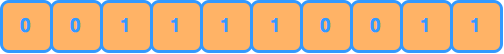
\includegraphics[width=3in]{img/onemax}
		\caption{Génome d'individu pour le problème \textit{one max}.}
	\end{center}
\end{figure}

\subsubsection{Initialisation}\label{initialisation}

Au début de l'algorithme, la population initiale est définie en créant
des individus aléatoires. Les GA nécessitent des générateurs de nombre
aléatoire uniforme rapide et de bonne qualité pour garantir un bon
échantillonnage de l'espace de recherche comme les générateurs
\emph{Mersenne twister} ou plus récemment les \emph{xorshift\cite{marsaglia2003xorshift}}. \\
Selon le problème, il peut se révéler intéressant d'introduire des
contraintes ou même des individus étant eux même des solutions de bonne
qualité pour aider la recherche. Ces biais ont néanmoins tendance à trop
contraindre les solutions possibles et à perdre la possibilité d'obtenir
des résultats créatifs.

\subsubsection{La boucle
évolutionnaire}\label{la-boucle-uxe9volutionnaire}

Après initialisation de la première population, la boucle évolutive
suivante va être répétée jusqu`à un critère de terminaison ou
indéfiniment dans le cadre d'une optimisation dynamique Anytime. Une
itération de la boucle par analogie au monde de la biologie est appelée
génération.

\begin{figure}[htbp]
	\begin{center}
		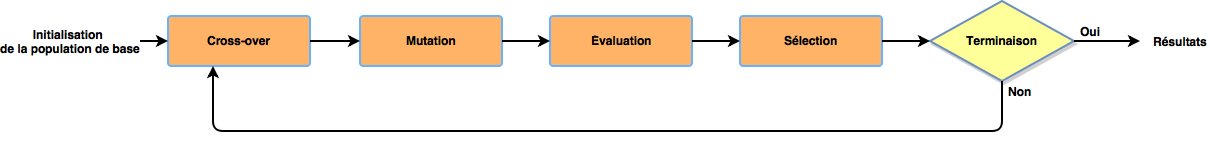
\includegraphics[width=6in]{img/gen_loop.png}
		\caption{La boucle évolutionnaire d'un algorithme génétique.}
	\end{center}
\end{figure}


\subsubsection{Évaluation}\label{uxe9valuation}

La fonction d'évaluation est la partie la plus importante des GA étant
donné qu'elle va guider l'évolution vers des solutions de plus en plus
efficaces. Elle permet de « noter » un individu par rapport au problème.
Cette note représente la fitness de l'individu. \\
La fonction d'évaluation représente l'espace de recherche et décrit le
paysage de \emph{fitness} (fitness landscape) en l'échantillonnant et
l'extrapolant grâce à une population d'individu. « Graphiquement »,
l'algorithme cherche à découvrir les endroits les plus intéressants de
son espace de recherche.

\begin{figure}[htbp]
	\begin{center}
		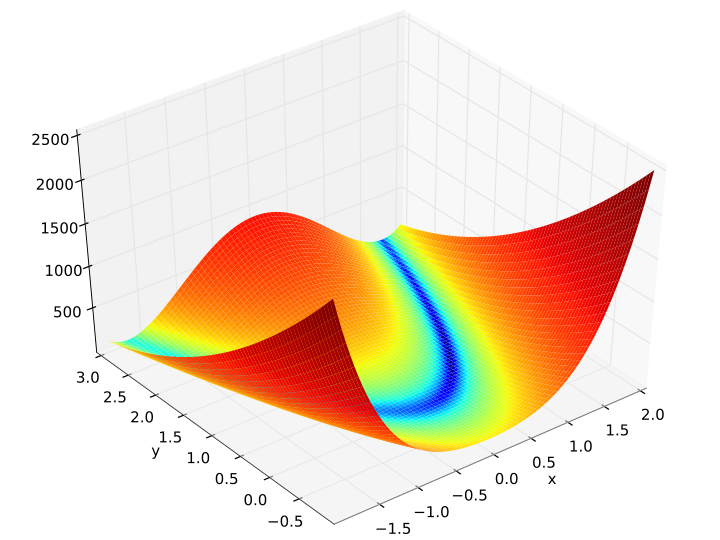
\includegraphics[width=4in]{img/fitnessLandscape.png}
		\caption{Paysage de fitness d'une fonction de Rosenbrock.}
	\end{center}
\end{figure}


\subsubsection{Cross-over}\label{cross-over}

La phase de \emph{crossing-ove}r (ou recombinaison, reproduction)
consiste à créer de nouveaux individus d'après plusieurs parents. De
nombreux types de \emph{cross-overs} existent, adaptés à diverse
représentation d'individu. Le cross-over doit prendre en compte la
structure de l'individu et est de fait lui aussi spécifique au problème.

\subsubsection{Mutation}\label{mutation}

L'opérateur de mutation permet de faire varier de manière aléatoire les
nouveaux individus « enfants » pour améliorer l'exploration de l'espace
de recherche, certaines « zones » ne sont potentiellement pas
accessibles par \emph{cross-over} ou lorsqu'il n'y a pas eu d'occurrence
d'un gène ou d'une certaine valeur d'un gène dans la population
initiale. Là encore, l'opérateur de mutation dépend du problème et de la
représentation utilisée, par exemple de l'ajout de bruits dans le cas
d'un problème continu ou des opérations de swapping dans le cadre
combinatoire.

\subsubsection{Sélection et
réduction}\label{suxe9lection-et-ruxe9duction}

Avant d'entamer la prochaine génération, il faut assigner les « nouveaux
» parents d'après l'ensemble ($\lambda$ + $\mu$) des individus enfants
$\lambda$ et des parents $\mu$ de la génération précédente. Le nombre
d'individus sélectionnés de cette manière est égal à la taille
originelle de la population parent $\mu$. \\
La sélection se base sur la \emph{fitness} des individus. Cependant, un
mécanisme simpliste où seuls les meilleurs (les plus aptes) individus
sont sélectionnés, après un tri par exemple, entraîne des problèmes de
convergence prématurée.

\bigskip
Lors du processus de sélection, il est nécessaire de garder des
individus ``relativement\cite{sharma2010archived,deb2002fast}'' bons qui aident à maintenir une certaine
diversité dans la population globale, ce qu'un choix déterministe ne
garantit pas. \\
Les méthodes de sélection sont donc généralement stochastiques comme la
très courante et efficace sélection par tournoi, qui retourne le
meilleur individu d'un ensemble aléatoire de n éléments. 
Il est à noter que les méthodes de sélection, ou sélecteurs diffèrent
grandement entre une \emph{GA} simple et une optimisation multicritère
(\emph{MOEA\footnote{Multi Objective Evolutionary Algorithm}}). Ce point précis sera bordé dans la section suivante.

\subsubsection{Optimisation
multiobjectif}\label{optimisation-multiobjectif}

L'intérêt d'utiliser des algorithmes génétiques vient que les résultats
obtenus sont créatifs et compétitifs avec l'intelligence humaine. Au
bout d'un certain nombre de générations, et ce malgré le fait d'avoir
initialisé les individus aléatoirement, on obtient de « bons »
résultats. On les définit comme « bon » du fait qu'on ne peut pas
déterminer si l'optimum global du problème a été atteint ou si
l'optimisation est restée bloquée dans un optimum local. Classiquement,
on cherche à optimiser un seul critère, mais il est aussi possible d'en
avoir plusieurs possiblement antagonistes. La difficulté des algorithmes génétiques multiobjectifs (\emph{MOEA}) vient de l'opérateur de
sélection. 
\\ Dans le cas d'un algorithme mono-objectif, la sélection se
fait de manière relativement évidente : on prend les meilleurs individus
issus de multiples tournois. Avec un MOEA, comment définir un « bon »
individu ? Un individu optimisant parfaitement le critère 1 et pas les
autres est-il meilleur qu'un autre qui optimise moyennement tous les
critères ? Le principe derrière tous les opérateurs de sélection
multiobjectif (\emph{NSGA-II\cite{deb2002fast}, ASREA\cite{sharma2010archived,sharma2010gpgpu}, SPEA}) nous vient du monde de
l'économie. Il s'agit de l'optimalité de \emph{Pareto}, aussi appelée
\emph{Pareto-dominance}.

\paragraph{Dominance de Pareto}\label{dominance-de-pareto}

Dominer au sens de Pareto\cite{voorneveld2003characterization}, pour un élément donné, signifie qu'aucun
autre élément n'a au moins un critère meilleur que les siens. Dans le
cadre des \emph{MOEA}, une solution domine une autre si les deux
conditions suivantes sont remplies:

\begin{itemize}
\item
  La solution x1 n'a aucune fitness plus mauvaises que celle de x2
\item
  La solution x1 a au moins une fitness meilleure que celle de x2
\end{itemize}

\begin{figure}[htbp]
	\begin{center}
		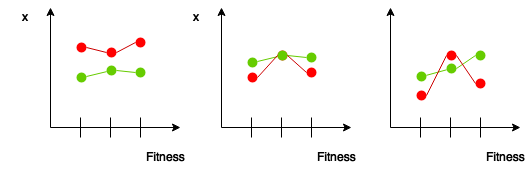
\includegraphics[width=4in]{img/paretoDominance.png}
		\caption{Soit deux individu, rouge et vert. Pour un problème de minimisation, de gauche à droite, vert domine rouge, rouge domine vert et ni rouge ni vert ne se dominent.}
	\end{center}
\end{figure}


% Plus formellement: // formule en laTex

De par cette définition on peut déduire le concept de \emph{front de
Pareto}: l'ensemble des solutions non dominé. Les fronts de Pareto
permettent de trouver de bons compromis entre les différents objectifs.
Définir un front de Pareto revient à trouver une enveloppe convexe\cite{godfrey2007algorithms} dans
un espace à dimension \textit{n}, où \textit{n} est le nombre d'objectif.


\begin{figure}[htbp]
	\begin{center}
		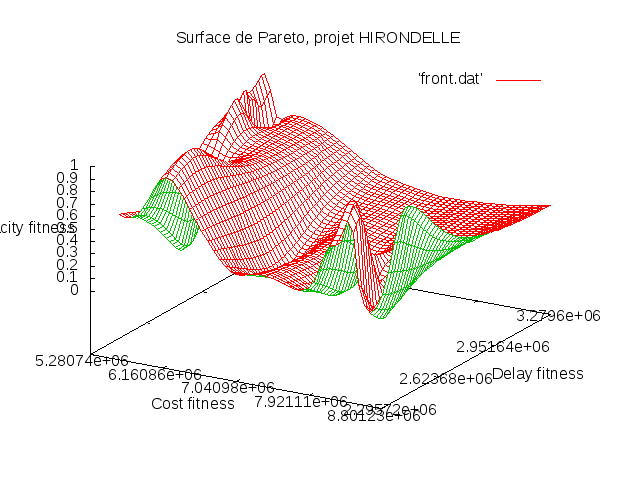
\includegraphics[width=4in]{img/paretoSurface.png}
		\caption{Surface de Pareto tiré d'HIRONDELLE à la génération 57.}
	\end{center}
\end{figure}

\section{EASEA, un framework évolutionnaire}

Dans le cadre de la finalisation d'un papier de recherche ayant pour
thème la « \emph{Musicalisation\cite{lutton2014visual}} » d'écosystème de calcul financé par le
projet \emph{EASEA-CLOUD}, plus tard publié dans le « \textit{Journal of grid
computing} », j'ai passé le premier mois d'alternance au CNRS à
corriger et compléter les demandes et questions de rapporteurs
scientifiques. Les coauteurs faisant principalement partie de l'équipe
\textit{BFO} et de l'équipe \emph{UMR3695 BioEmergences} à l'Institut des
Systèmes Complexes à Paris, une grande partie de la collaboration s'est
faite au travers d'email. \\
Le niveau de qualité demandé se traduisait par un travail précis,
documenté et techniquement irréprochable.

\subsection{Contribution}\label{contribution}

Le développement sur la plateforme EASEA a été assez libre : c'est au
cours de réunions d'équipe \emph{SONIC}, organisé tous les 2 mois compte
tenu de la disponibilité et de l'éloignement géographique de certains
intervenants que la \textit{roadmap} a été dressée. Une grande partie de cette
roadmap, axée sur la parallélisation automatique complète sur CPU et
carte \textit{GPGPU}, est du fait de mon initiative après plusieurs discussions
communes avec mon maître de stage de l'époque M. Collet. Cette prise de
position venait du fait d'avoir travaillé pendant les six mois
précédents sur le projet et connaissants parfaitement la
\emph{codebase}. \\
Sous l'égide du projet \emph{EASEA-CLOUD}, je m'occupais de continuer le
développement sur la plateforme elle-même.

\subsubsection{Flex/Bison}\label{flexbison}

Une mise à jour importante du compilateur \emph{EASEA}, concernant
l'analyse syntaxique et lexicale, qui embarquait de vieilles
technologies propriétaires payantes et abandonnées uniquement
disponibles sous \emph{Windows}, s'est révélé nécessaire. \\ Vétustes et
obsolètes, elles impliquaient un workflow de développement très
compliqué, nécessitant une compilation en plusieurs temps, sous Windows
pour la génération des parseurs et sous Linux pour le reste du projet. 
Elles ont été remplacées en faveur d'outils standards dans le domaine de
la compilation, \emph{Flex\footnote{http://flex.sourceforge.net/}} (analyseur lexical) et \emph{Bison\footnote{http://www.gnu.org/software/bison/}}
(analyseur syntaxique), multiplateformes, robustes, activement mis à
jour et suivis. \emph{Flex }(\emph{fast lexical analyzer generator}) est
un logiciel de génération d'analyseurs lexicaux en \textit{C/C++} tandis que
\emph{Bison} est un logiciel de génération de parseur en \textit{C/C++}. \\ Cette
modification a été effectuée par un contributeur tiers, et ensuite
intégrée après tests et vérifications.

\subsubsection{Nettoyage de la codebase}\label{nettoyage-de-la-codebase}

Des fonctionnalités diverses, issues de stages, de thèses et de postdoc
ont été testées puis intégrées à \emph{EASEA}, dont le \emph{tracking}
de la généalogie des individus. \\
De nombreux chercheurs, stagiaires, thésards et contributeurs tiers ont
participé à ce grand projet universitaire au cours des dix dernières
années. Des problèmes de style et de performances découlaient du manque
de travail d'uniformisation du projet. Un travail de normalisation sur
la cohérence du style et de la présentation du code s'est avéré
essentiel avant de continuer les travaux sur le projet.

\bigskip
Les parties critiques touchant aux performances de la bibliothèque
\emph{EASEA} ont été \emph{refactoré }pour en améliorer la lisibilité,
notamment pour la boucle génétique en elle-même. Une amélioration de la
gestion mémoire lors de la déclaration des structures utilisateurs liées
au génome, plus permissive et poussée, liée au support de l'arithmétique
des pointeurs a aussi été intégrée. C'est notamment cette partie qui
posait de nombreux problèmes aux premiers prototypes du projet
HIRONDELLE pendant le séjour de M. Catania. Nous avons travaillé
ensemble sur ce nouveau système de gestion du génome. \\
La base de code a été nettoyée de quelques bugs critiques qui nuisaient
à la stabilité du système dans son ensemble. Ils étaient en particulier
présents dans la gestion des paramètres utilisateurs (choix du port de
connexion, choix des pressions de sélection et de réduction) et dans la
couche de communication réseau entre les instances. D'autres bugs et
malfonctionnement plus légers ont aussi été corrigés lors de l'étape de
refactorisation.

\bigskip
Garantir la stabilité d'un tel framework est primordial pour qu'il soit
utilisé pour des projets commerciaux ou universitaires de grande
envergure, comme dans le cas d'HIRONDELLE.
Le projet EASEA-CLOUD à vocation à être déployable sur toutes les
plateformes et architecture. Un gros point noir du projet était le
manque de pour support pour le système d'exploitation Windows. \\
Le portage
d'\emph{EASEA} vers \emph{Windows} a été réalisé avec succès. Il
nécessite l'utilisation de \emph{MinGW}. \emph{MinGW\footnote{www.mingw.org/}} (\emph{Minimalist
GNU for Windows}) qui est un environnement de développement pour Windows
incluant une toolchain de compilation \textit{C/C++} basée sur GCC. De par les
efforts entrepris sur l'utilisation multiplateforme, \emph{EASEA }est
maintenant nativement disponible sur \emph{Windows}, \emph{Linux} et
\emph{OSX}.

\subsubsection{Visualisation}\label{visualisation}

Un début de travail sur des visualisations complexes de diverses
métriques a été entrepris. Il s'agit pour l'instant d'une visualisation
de la généalogie des individus en utilisant la bibliothèque
\emph{JavaScript} \emph{D3.js}. \emph{D3.js\footnote{http://d3js.org/}} (\emph{Data driven
document}) est une bibliothèque JavaScript de visualisation dynamique et
interactive de données se basant sur les capacités des navigateurs Web à
gérer les standards \emph{SVG} (dessin vectoriel), \emph{HTML5} et
\emph{CSS}. \\
L'intérêt de ce développement était d'évaluer la possibilité
d'utiliser directement des technologies issues du Web, en particulier au
niveau du rendu visuel, dans le but d'une intégration plus profonde avec
le fonctionnement sur le cloud. Les différents graphiques et
visualisations des instances \emph{EASEA-CLOUD }pourraient donc être
servis directement sur navigateur, facilitant là encore une prise en
main massive et rapide de la plateforme. 

\bigskip
Pour HIRONDELLE nous avons utilisé les mêmes technologies et idéologies.
Toutes les visualisations (front de Pareto, courbe d'évolution des
fitness et représentation spécifique au problème) sont disponibles
directement sur un browser. \\
L'ajout d'un système de visualisation (et d'exportation automatique
liée) modulaire et générique reste une des fonctionnalités importantes à
ajouter à EASEA pour en faire un outil complet.

\subsubsection{Industrialisation}\label{industrialisation}

Un des buts de ce CDD était de faire d'EASEA un outil facilement
utilisable et déployable, et utilisé, nous avons donc entamé un
processus d'industrialisation pour faire de la plateforme un outil de
qualité professionnelle.

\bigskip
Une première tâche importante consistait à mettre à jour \emph{EASEA}
pour supporter les nouvelles versions des \emph{SDK\footnote{Software Development Kit} CUDA}, les
bibliothèques de développement sur cartes \emph{GPGPU} de marque
\textit{NVIDIA}, en particulier pour les versions supérieures à 4. Le
support des versions récentes de CUDA a apporté de la flexibilité et des
améliorations de performances au niveau du calcul sur carte
graphique. \\
Sur le même principe, une migration vers des versions du
compilateur \textit{C++ GCC} plus récentes, toujours dans un but d'avoir un
outil le plus facilement et universellement déployable, a été
entreprise. \emph{EASEA} étant multiplateforme, le support d'autres
compilateurs que \emph{GCC} notamment \emph{Clang}, compilateur préféré
sous Mac OSX, a été amélioré. EASEA reste néanmoins un outil universitaire s'appuyant sur la
contribution de chercheurs et passionnées à travers le monde.

\bigskip
Le code d'EASEA à donc était mis sur \emph{Github\footnote{https://github.com/}}, qui est devenu en
2014 le plus grand hébergeur de code au monde et qui propose des outils
collaboratifs efficaces. \emph{Github} est un service Web, gratuit pour
les projets de type « open source », qui se présente comme une interface
des fonctionnalités du système de versionnage décentralisé Git, en plus
de ses propres outils de gestion de projet (permissions, \emph{tracker}
de bug, canaux de discussion). Ce choix se justifie premièrement par la
présence de fonctionnalités et d'outils de travail collaboratif qui se
trouvent être spécialement adaptése au projet, regroupant des équipes et
laboratoires répartis sur tout le territoire. Cette plateforme
d'hébergement de code jouit aussi d'une excellente visibilité dans le
milieu du développement du logiciel libre et permet de mieux faire
connaître la plateforme \emph{EASEA-CLOUD}, tout en attirant de
possibles tiers contributeurs. \\
Des efforts soutenus de documentation ont été fournis concernant
l'accessibilité du code source du projet \emph{EASEA-CLOUD}, qui
s'inscrit dans la longue tradition du logiciel libre. Le code source du
compilateur et de la bibliothèque EASEA a été entièrement documenté selon
la nomenclature du système de documentation \emph{doxygen}, qui est le
standard pourle développement \emph{C/C++}. Le code source du projet
principal, ainsi que des projets annexes de « musicalisation »
\emph{musEAc} et de visualisation \emph{GridVis} sont maintenant
disponibles et hébergé sur la plateforme \emph{Github}. \\
De plus, le processus d'installation et de déploiement a été largement
simplifié etautomatisé. Des systèmes de compilation avancés ont donc été
mis en place. Le projet EASEA utilise désormais \emph{Cmake\footnote{www.cmake.org/}} pour la
compilation de la plateforme.\emph{Cmake} est un système de compilation
multiplateforme et qui permet de s'affranchir des spécificités des
différents systèmes d'exploitation. Il nécessite le moins de dépendances
possible, le rendant \emph{de facto} très flexible et tout indiqué au
développement multiplateforme.

\bigskip
Toujours dans un but d'offrir une plateforme stable et pérenne, l'ajout
de script type bash permet au développeur travaillant sur
\emph{EASEA-CLOUD} d'effectuer des \textit{tests de régression},
indispensable pour tester le bon fonctionnement de la base de code après
une intégration ou une modification de fonctionnalités. \\
La base de code a
aussi été analysée grâce à des outils d'analyse statique
(\textit{clanganalyzer}), de graphe d'appel pour détecter les « \textit{hotspots}
» (\emph{callgrind}) et valgrind\footnote{valgrind.org/} pour détecter d'éventuels problèmes
liés à la gestion de la mémoire.

\subsubsection{Parallélisation CPU}\label{paralluxe9lisation-cpu}

La première grosse amélioration apportée au cours de ce CDD fut l'ajout
de multithreading complet sur \textit{CPU} de la boucle évolutionnaire. \textit{EASEA}
propose depuis plusieurs années de la parallélisation automatique sur
carte \textit{GPGPU} mais n'en proposait aucune sur processeurs, beaucoup plus
courants. Dû aux spécificités de l'architecture \textit{CUDA} expliquée en détail
dans la section précédente, tous les projets n'en tirent pas forcément
parti, voire ont des performances inférieures à une exécution
séquentielle sur \textit{CP}U.

\bigskip
Une initiative de parallélisation sur \emph{CPU}, se basant sur la
bibliothèque \textit{OpenMP}\footnote{http://openmp.org}, a porté très rapidement ses fruits en
obtenant en quelques semaines une version d'\textit{EASEA} avec tous les
opérateurs génétiques parallélisés (évaluation, croisement, réduction et
mutation). \\
\emph{OpenMP} est une \emph{API\footnote{Application Programming Interface}} de programmation multicœur à modèle de
mémoire partagée en \textit{C/C++} et \emph{Fortran}. \emph{OpenMP} fournit une
\emph{API} portable et simple d'utilisation.

\section{La plateforme Web du CSDC}\label{la-plateforme-web-du-csdc}

J'ai aussi travaillé en étroite collaboration avec M. Collet et M.
Bourgine sur le système informationnel du \emph{Campus Numérique des
Systèmes Complexes}. \\
L'aventure du CSDC s'est montrée instructive sur de nombreux points, en
bien comment en mal. En étroite collaboration avec M. Pierre Collet et
M. Paul Bourgine, les initiateurs du projet et M. Rudolf Dietrich ,
développeur, les échanges furent nombreux. La disponibilité en journée
des différents interlocuteurs faisant que la plupart de réunion de
travail ont eu lieu après les horaires de travail habituels, le jeudi
soir. Il est intéressant de noter que le système fonctionne sur la base
d'une hiérarchie floue où toutes entités peut être rattachée une autre
(cf.~fig 1). Cela a pour but de favoriser les échanges transversaux
entre différentes équipes de recherche, tant bien même qu'elles fassent
partie de filières différentes.

\bigskip
Le projet était encore très vague dans ses débuts, donnant lieu dans des
spécifications particulièrement mouvantes. Avec du recul ce début de
projet s'apparenté très fortement à un travail de recherche: les
modélisations de la hiérarchie floue que devait proposer la plateforme
Web du CSDC en est un bon exemple. \\
Les différentess types d'entités du CSDC sont les suivantes:

\begin{itemize}
\item
  E-Departement
\item
  E-Lab
\item
  Project-Team
\item
  Ressources
\item
  Commitee
\item
  Individual member
\end{itemize}

\bigskip
Chacun de ces types d'entités se caractérise au minimum par un nom, un
représentant, responsable scientifique, une description du projet
scientifique de l'entité et une liste de membre. À cela s'ajoutent des
informations complémentaires: co-représentant, liste de mot-clé et
d'autre information liée au type lui-même. \\
Plus formellement, les entités du csdc forment un treillis avec une
relation d'ordre partielle sur leurs types. Ces interactions étant trop
nombreuses à décrire, le tableau décrivant cette relation d'ordre et
disponible en annexe.

\subsection{Python et framework
Django}\label{python-et-framework-django}

Venant sur un projet en ne connaissant ni le langage ni le
\emph{framework} Web \emph{Django}, j'ai rapidement appris le
fonctionnement de ces deux derniers grâces à leurs documentations très
fournis et illustrés ainsi que par l'aide la communauté \emph{Python} \&
\emph{Django}, très présente sur internet. \\
Je me suis familiarisé avec la \emph{codebase}, déjà très volumineuse du
projet ainsi qu'avec l'architecture \emph{MVC\footnote{Model–View–Controller}}du \emph{Django}.
L'apprentissage de l'\emph{ORM\footnote{Object-relational mapping}} a été un peu plus long, dû à sa
complexité.

\subsection{Contribution}\label{contribution-1}

\subsubsection{Mise en place d'un système de templating de
mail}\label{mise-en-place-dun-systuxe8me-de-templating-de-mail}

Une des problématiques rencontrées était que la plateforme Web devait
être capable d'envoyer un certain nombre de modèle d'emails , et que les
modèles doivent pouvoir être modifiés rapidement par les différents
acteurs de la plateforme. \\
En effet, un représentant d'une entité interconnectée à d'autre de
niveaux hiérarchique plus faible, peut envoyer des emails aux différents
membres les constituants.

\bigskip
Une interface sous forme d'application Web complètement générique
épaulée par une petite API \emph{RESTFul\footnote{Representational State Transfer}} permettant aux administrateurs
de la plateforme de modifier rapidement le type et contenu des emails
envoyés suite à certains événements définis en interne été mise en
place. \\
Le développement du système de templating d'émail s'est fait sans l'aide
de bibliothèques tierces, qui après recherche minutieuse ne
correspondaient pas aux exigences du projet de généricité et de
flexibilité du projet.

\subsubsection{Exportation/importation
Wikiversity}\label{exportationimportation-wikiversity}

La plateforme du \emph{CSDC} se veut la plus ouverte et transparente
possible. Il a donc été décidé de mettre en place un système
d'import/export des différents contenus, formulaires et descriptifs
d'entité vers le portail \emph{Wikiversity} du projet. Le projet
\textit{Wikimedia\footnote{https://www.wikimedia.org/}}, le \textit{CMS\footnote{Content Management System}} derrière \emph{Wikipédia} et ses sites
satellites, fournit un \emph{bot} en \emph{Python} pour faciliter les
création et édition de pages automatiques. \emph{Pywikibot} est facile
de prise en main, une fois l'architecture et les tags de site
\emph{Wikimedia} compris. \\
Des guidelines quant à l'utilisation d'outils
automatisés sont à respecter, tel que la fréquence de mise à jour,
l'utilisation d'un compte avec des autorisations spécifiques validées
pour un administrateur, et la présence de tags indiquant la nature du
robot et de ses changements dans les messages de commit des articles.

\subsubsection{Visualisation}\label{visualisation-1}

Développement d'interface graphique novatrice pour
expliciter la complexité du système (liens entre les différentes
entités) tout en restant lisible et compréhensible. Ces différentes
visualisations se basent sur la librairie \emph{JavaScript D3.js}, déjà
évoquée plus haut et \emph{OpenLayer\footnote{openlayers.org/}} pour la partie cartographie. Elles
se sont montrées assez rapidement nécessaires une fois une première
phase de \emph{beta-testing}, le nombre d'entités et leurs
interconnexions ayant alors significativement augmenté.\\ 
Ces visualisations sont aux nombres de trois :

\paragraph{Cartographie Map}\label{cartographie-map}

Création d'une carte avec \emph{OpenLayer} et fonds de cartes
\emph{OpenStreetMap} pour répertorier géographiquement les institutions
et les équipes de recherches affiliées. Ne manipulant que des adresses
postales, le service de geocoding \emph{Nominatim\footnote{https://nominatim.openstreetmap.org/}} du projet
\emph{OpenStreetMap} a été utilisé. Là encore, les règles de bonne
utilisation de l'\emph{API} publique à du êtres respecté, notamment le
taux de requête par seconde. Une fois les informations \emph{GPS} d'une
adresse obtenues celle-ci est mise en base pour améliorer les performance pendant la navigation.

\begin{figure}[htbp]
	\begin{center}
		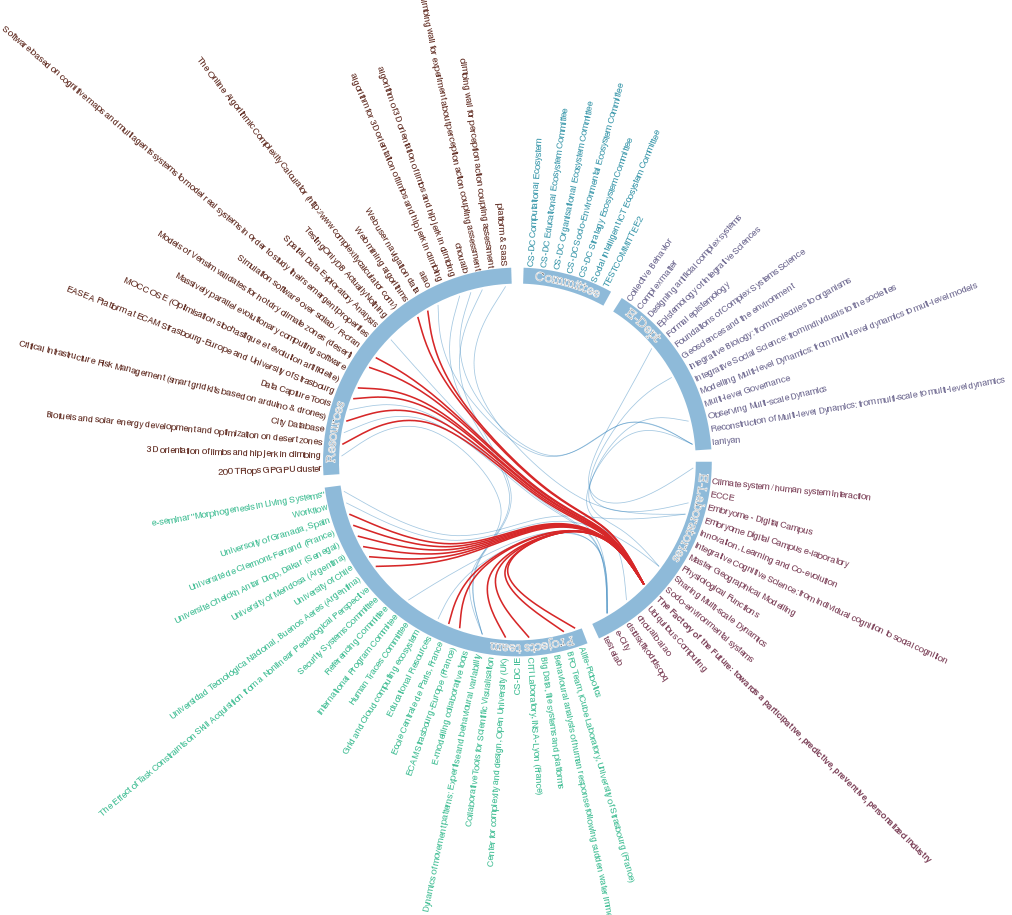
\includegraphics[width=4in]{img/csdcDaisy.png}
		\caption{Représentation par \textit{Hierarchical Edge Bundling} des interconnexions des entité du \textit{CSDC}.}
	\end{center}
\end{figure}

\paragraph{Marguerite}\label{marguerite}

La visualisation des interconnexions entre entités du \emph{Campus
numérique des Systèmes complexes} se fait à travers une «\textit{ marguerite} ».
Il s'agit d'une technique de visualisation récente appelée «
\emph{Hierarchical Edge Bundling\cite{holten2006hierarchical}} » dont la qualité première est
d'offrir une vue d'ensemble de graphe fortement connexe. Il s'agit d'un
module proposé par \emph{D3.js}.


\paragraph{Matrix}\label{matrix}

La navigation à travers les entités du csdc a posé un véritable souci
d'ergonomie. Pour pallier à cela, une matrice entre les éléments de
niveaux hiérarchiques égale à prouver son efficacité. Entièrement en
\emph{JavaScript}, elle se base sur \emph{Jquery}.

\subsubsection{Notification interne}\label{notification-interne}

De très nombreuses interactions requièrent des validations utilisateurs.
Un système de notification interne au site a été mis en place, pour
pouvoir gérer en une partie les \emph{use-cases} suivant : des
interactions entre les différentes entités (demande de rattachement,
description incomplète, etc.) et utilisateurs.
Des
notifications de plusieurs types sont supportées comme des modales
(boutons de choix) ou infobulles.\\
 Là
encore, les bibliothèques et autres modules \emph{Django} de
notification se sont révélés peu adaptés aux besoins de la plateforme,
ce qui nous a poussés à développer notre système \emph{ex nihilo}.

\subsubsection{Modélisation}\label{moduxe9lisation}

Le projet étant déjà bien entamé, les ajouts de fonctionnalités
nécessitèrent d'être intégré avec soin à la base de données existante. Le
projet étant sous \emph{Django} 1.6, les migrations automatiques
n'étaient pas encore disponibles avec la base \emph{PostgreSql} en
production. Le module de migration \emph{South} avait vocation à être
ajouté au \textit{workflow} de développement, facilitant les changements
sur les modèles de données internes. \\ 
PostgreSql et ses outils associés de visualisations ont aidé à réduire la taille 
et la complexité de la base de données, tâche de fond pendant toute la durée du projet. Le
cycle de développement très rapide, parfois seulement une journée de la
conception à la mise en production, à souvent causé problème avec le
workflow de modification de la base de données, requièrent souvent une
intervention manuelle.

\subsubsection{Refactoring}\label{refactoring}

Des outils de refactoring et d'aide à la qualité de code performant ont
été utilisés dans un premier mouvement de nettoyage de la codebase tels
que \emph{Pylint}, \emph{pyStorm}, et la convention
\emph{Pep8}. \emph{Pylint} est un analyseur statique de code qui indique
les mauvaises pratiques : fonctions trop longues, complexité
cyclomatique élevée, variable utilisée sans être initialisée. De plus
\emph{Pylint} offre une analyse de la duplication de code et prodigue
des conseils pour suivre la méthodologie \emph{DRY} (\emph{Don't repeat
yourself}) très chère à la communauté Python. \\
\emph{Pylint} incorpore
avec un module de vérification de style \emph{pep8\footnote{https://www.python.org/dev/peps/pep-0008/}} : ligne trop longue,
nom de variable mal formé, importation de modules inutiles. \textit{Pep8} est
la convention de code \emph{Python} standard, qui tire sa philosophie du
fait que le code est plus souvent lu qu'écrit. 

\bigskip
Ces outils ont permis de
corriger des bugs jusqu`alors non détectés et d'améliorer la lisibilité
du code tout en facilitant le \emph{refactoring}, nécessaire sur un
projet aussi verbeux (\textgreater{} 30K \textit{loc}\footnote{1 KLOC : 1,000 ligne de code}). Le refactoring à
proprement parlé s'est fait grâce à \emph{pyStorm}, un \emph{IDE\footnote{Environnement de développement}} payant
offert aux étudiants au travers du programme d'aide aux étudiants de
\emph{Github}.

\section{Le projet HIRONDELLE: Spécialisation poussée sur les techniques
évolutionnaires et l'architecture
CUDA}\label{le-projet-hirondelle-spuxe9cialisation-poussuxe9e-sur-les-techniques-uxe9volutionnaires-et-larchitecture-cuda}

J'ai continué ce projet de R\&D en me basant sur les travaux effectuer
par le dernier développeur et post-doctorant ayant travailler dessus,
Carlos Catania toujours dans le cadre de la collaboration entre
\emph{Synovo} et le laboratoire \emph{ICube}. \\
Étant déjà familiarisé avec
le travail de Carlos lors de mon stage dans l'équipe \emph{BFO} qui
s'est déroulé de début février à juillet 2014 sur le projet
\emph{EASEA}, j'avais une bonne compréhension des différents éléments du
projet. \\
Les problématiques techniques rencontrées étaient les suivants :
problèmes de gestion de la mémoire entre le système et les cartes
\emph{GPGPU}, le manque d'implémentation d'algorithmes efficaces pour
gérer les critères multiples ainsi que le fait que l'algorithme en
lui-même n'est pas complètement finalisé.

\bigskip
J'ai récupéré de M. Catania
l'intégralité de ses notes, comptes-rendus de réunion ainsi que touts le
code développé durant le déroulement de son postdoc en \textit{BFO} :
prototypes divers, expérimentations, etc. Un prototype fonctionnel était
déjà disponible et fournissait des résultats allant dans la bonne
direction malgré le fait qu'il n'intégrait pas toutes les contraintes et
données du problème. \\
L'implémentation a été faite sur la plateforme
\emph{EASEA} et correspond à environ 5K \emph{loc} de \emph{C++}. Le
prototype fonctionne en version \emph{CPU} parallélisée et en version
\emph{CUDA} massivement parallèle. Entre la version \emph{CPU} et
\emph{CUDA}, l'implémentation \textit{CUDA} était trois fois plus lente. Ceci
était dû à plusieurs raisons : l'empreinte mémoire du génotype qui
entraînait des tailles de populations importantes (plusieurs
\emph{gigaoctets} pour quelques milliers d'individus) et code des
opérateurs non optimisés pour le traitement sur \textit{GPGPU}. Cependant, la
qualité des résultats expérimentaux obtenus était satisfaisante.

\subsection{Description fine du
problème}\label{description-fine-du-probluxe8me}

\subsubsection{Problématique}\label{probluxe9matique}

Comme énoncé en introduction, la problématique est de fournir une
tournée de véhicules sanitaire en réduisant les coûts de fonctionnement,
la durée de la planification (temps d'utilisation des véhicules et
employé) et en maximisant des contraintes de qualité de
service. L'algorithme doit ensuite être intégré à \textit{Saphir}, la
solution de Synovo pour les sociétés et services de transport
ambulancier. Dans un premier temps, l'optimisation se fait de manière
ponctuelle. À l'appui sur un bouton dans l'interface de régulation, les
données des missions journalières sont sérialisées et exportées sur le
serveur d'optimisation qui lance alors le calcul.\\
L'utilisateur, une
fois le processus d'optimisation entamé peut alors récupérer à tout
moment une planification complète de la journée. Il est à noter que dû à
sa nature d'algorithme d'optimisation non déterministe évolutionnaire,
les résultats obtenus pendant les premières générations d'hirondelle
sont d'assez mauvaise qualité. Au fil des générations, la qualité des
résultats s'améliore grandement. \\
Le projet correspond à des problèmes
d'optimisation de type « \textit{vehicle routing problem} » (VRP),
sujet dont la littérature académique est riche\cite{kallehauge2005vehicle,toth2001vehicle,kallehauge2005vehicle} et ayant déjà ses
variantes propres au monde de la santé, regroupées sous les coupes des «\textit{
healthcare management science} ». Nous nous situons sur modèle de type «
\textit{Delivery pickup vehicle routing problem with time windows\cite{solomon1987algorithms,kallehauge2005vehicle,ombuki2006multi}} »
(\emph{DPVRPTW}), vu que les patients doivent être récupérés et délivrés
à une heure précise. Une recherche exhaustive n'est pas possible dû à la nature combinatoire
du problème, \textit{NP-Complet\cite{gendreau2008metaheuristics}}.

\bigskip
Nous proposons donc une résolution par algorithme génétique multicritère
optimisant le coût du planning, les délais d'attente et de retard pour
les patients et certaines contraintes de qualité de service décrite dans
la section suivante. \\
L'idée innovante derrière \emph{HIRONDELLE} est
qu'il s'agit d'un algorithme dit \emph{Anytime}. Peu importe quand
l'utilisateur demande une solution, l'algorithme va à tout moment
renvoyer une réponse valide, et va continuer à améliorer ses résultats
avec le temps. De surcroit, l'optimisation est dynamique : le problème à
optimiser va changer avec le temps en prenant en compte les réalités du
terrain : Retard sur une mission, annulation, changement d'horaire. Des
résultats théoriques ont montré la grande résilience et flexibilité des
processus évolutionnaires avec des problèmes interactifs\cite{cho2002towards,hanshar2007dynamic,branke1999evolutionary}, ce qui nous a
naturellement poussés vers cette branche des méthodes stochastiques
plutôt que certaines techniques plus répandues comme les recherches
taboues\cite{gendreau2008metaheuristics}.

\subsubsection{Transfert de données et
communication}\label{transfert-de-donnuxe9es-et-communication}

Les données du problème à optimiser sont créées et exportées par
\emph{Saphi}r sous forme de données binaires sérialisées sous format
protocolbuffer\footnote{https://developers.google.com/protocol-buffers/} de Google. Ce choix a été avant mon arrivée, sur le
prototype développé avec EASEA. J'ai décidé de gardé cette technologie
de par sa facilité d'utilisation et sa robustesse, ce qui en fait un
choix pertinent pour le projet.\\ 
\emph{Protobuf} est un système de
sérialisation de donnée développé par Google pour faciliter les échanges
de données structurées entre back-end. La désérialisation est
particulièrement rapide, \emph{Protobuf} n'incluant aucun système de
compression. Les descriptions des binaires \emph{Protobuf} suivent une
syntaxe simple et sont automatiquement gérées côté C\# par \emph{Saphir}
lors de l'exportation.

\begin{figure}[htbp]
	\begin{center}
		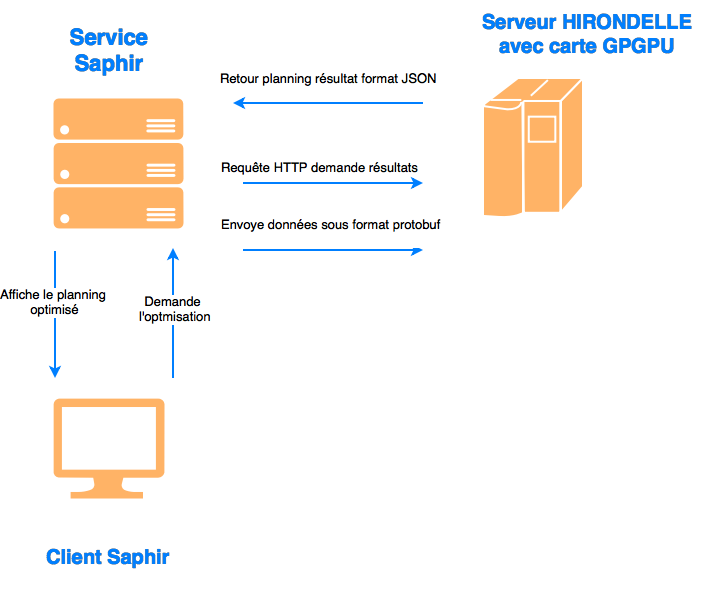
\includegraphics[width=5in]{img/communication.png}
		\caption{Description de l'architecture du projet.}
	\end{center}
\end{figure}


\subsubsection{Matrice de distance}\label{matrice-de-distance}

L'algorithme ne fait aucun calcul de distance et de durée entre les
adresses des missions, mais les récupère à travers une matrice
représentant le produit cartésien entre tous les points du problème.
Pour chaque adresse, on peut donc récupérer la distance en kilomètres et
la durée en secondes avec toutes les autres. Là aussi, la pertinence de
ce mécanisme m'a poussé à le garder, après un changement de structure de
données sous-jacente pour permettre plus facilement la mise à jour de
ses données et réduire son empreinte mémoire. \\
Ce cube est généré du côté
C\# par le back-office de \emph{Saphir} en s'appuyant du moteur de
cartographie \emph{PTV} qui calcule la durée et la distance entre deux
points de manière prévisionnelle d'après des statistiques de trafic
routier.

\subsubsection{Architecture de
données}\label{architecture-de-donnuxe9es}

S'agissant d'un projet de R\&D, la phase de prototypage a été assez
longue. Les modèles de données ont changé plusieurs fois d'avril à juin.
Voici une courte explication du data layout actuel :

\bigskip
Une mission (\emph{journey}) est composée deux \textit{planned element},
de type début et arrivée. La mission spécifie quels types de véhicules
doivent être utilisés et la facturation au client. \\
Un \textit{planned element}
est une description contextuelle liée une adresse : heure de passage
(\emph{timestamp UNIX}), identifiant d'adresse, type d'événement
(récupération ou dépôt de patient). Les véhicules ont une capacité de
passagers, un coût au kilomètre, un coût à l'heure ainsi qu'un type dont
découle certaines contraintes. Les quatre types de véhicules possibles
sont les suivants :

\begin{itemize}
\item
  VSL
\item
  TPMR
\item
  Ambulance
\item
  Taxi
\end{itemize}

\bigskip
Ces types ont des caractéristiques différentes : capacité, équipements
et taille de l'équipage requis. \\
Enfin, les employés ont un coût à l'heure définie par une fonction affine
par morceaux (\emph{piecewise}), et plusieurs types de diplôme et
certifications possibles. (licence de taxi, brevet de secourisme). \\
Cette \textit{piecewise} permet de nous abstraire de certains calculs plus
complexes, car elle prend en compte le nombre d'heures déjà travaillées
dans la semaine. Elle est aussi modifiée pour garantir certains
comportements par exemple si un employé ne peut commencer qu'après 10h,
on va assigner des valeurs arbitrairement hautes, pour qu'il ne soit pas
en charge d'une mission démarrant antérieurement.

\begin{figure}[htbp]
	\begin{center}
		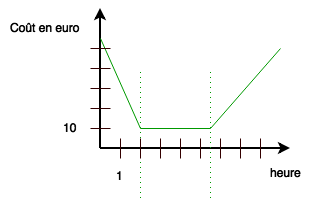
\includegraphics[width=2.5in]{img/piecewise.png}
		\caption{Fonction affine par morceaux (\textit{Piecewise function}) du cout d'un employé selon l'heure de la journée.}
	\end{center}
\end{figure}


\textbf{Génome }Le génome de nos individus (solution) est composé de
deux parties distinctes pour des raisons de facilitation des
manipulations par les opérateurs de \emph{cross-over}. \\
La première partie est un tableau contigu de \emph{Fare}, structure
référençant des éléments dans les données du problème pour réduire la
taille des populations. Une \emph{Fare} est constitué de référence par
index sur un \emph{planned Element}, deux employées et diverses données
qui elles sont redondante, pour d'optimiser les latences des accès en
mémoire globale sur GPU.

\begin{figure}[htbp]
	\begin{center}
		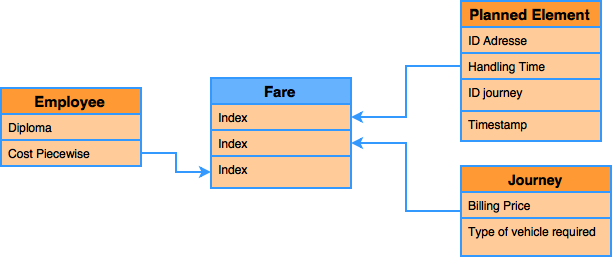
\includegraphics[width=4in]{img/Fare.png}
		\caption{Description d'une \textit{fare}.}
	\end{center}
\end{figure}

La deuxième partie est un simple tableau entier représentant la longueur
de la tournée de chaque véhicule. En parcourant ce tableau, on peut
connaitre l'offset à appliquer dans le premier pour accéder au
\emph{Fare} de chaque véhicule. \\
Cette représentation est justifiée par le fonctionnement de l'opérateur
de \emph{cross-over} \emph{\textbf{BCRC}\cite{ombuki2006multi}} utilisé.

\begin{figure}[htbp]
	\begin{center}
		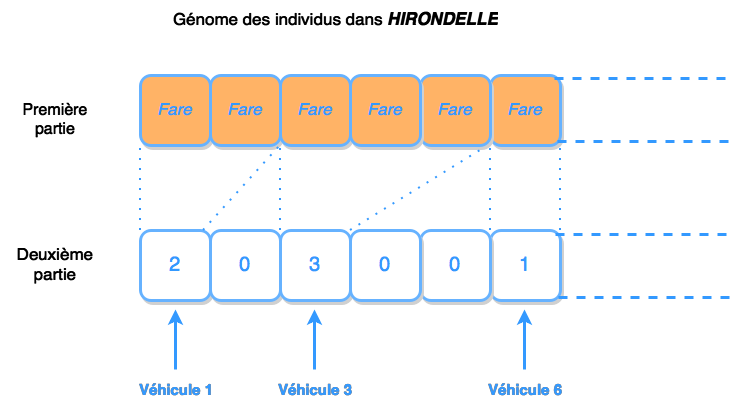
\includegraphics[width=5in]{img/individu.png}
		\caption{Génome des individu du projet \textit{HIRONDELLE}.}
	\end{center}
\end{figure}


\subsubsection{Constraintes}\label{constraintes}

Cette optimisation est considérée comme difficile par son caractère
multidimensionnel évoqué plus haut et les nombreuses contraintes à
prendre en compte. Le modèle \emph{Delivery-Pickup} utilisé, en plus des
contraintes de fenêtre de temps et de capacité, en fait un problème
\emph{NP-Complet}. \\
On en distingue de trois types de: contraintes « \emph{hard} », «
\emph{soft} » et les objectifs discrets.

\paragraph{Contraintes \emph{hard}}\label{contraintes-hard}

Les contraintes \emph{hard} représentent des cas de nullité d'une
solution. La violation d'une contrainte \emph{hard }signale une
incohérence ou une impossibilité physique rendant la solution non
exploitable:

\begin{itemize}
\item
  Mission assignée au mauvais type de véhicules
\item
  Véhicule en surcharge
\item
  Employé « \emph{ubiquitaire} », présence sur plusieurs véhicules
  simultanément
\item
  Pas de pause de plus de 20 minutes toutes les 6 heures pour une
  employée
\item
  Employé travaillant plus de 12 h par jour
\end{itemize}

\paragraph{Contraintes \emph{soft}}\label{contraintes-soft}


\begin{itemize}
\item
  Choix d'un VSL plutôt qu'un taxi pour les trajets de plus 9 kilomètres
\item
  Équipage roulant mixte
\item
  Employé ayant une mauvaise relation avec un client
\item
  Équipage ne parlant pas la langue d'un client
\item
  Équipage n'ayant pas le même nombre d'heures déjà travaillées
\end{itemize}

\paragraph{Objectifs discrets:}\label{objectifs-discrets}

Et les objectifs discrets :

\begin{itemize}
\item
  Le nombre de kilomètres parcourus
\item
  Les délais d'attentes ou de retards entre les missions
\end{itemize}

Pendant de l'évaluation, les malus associés aux différentes contraintes
sont agrégés aux différents objectifs. Ici, le tableau des deux échelles
de contraintes:

\begin{center}
\begin{tabular}{ |l| c| r| }
		\hline
	Type Contraintes & Borne inférieure & Borne supérieure \\
	\hline
	Forte (hard) & 50 000 & 5 000 000 \\
	Faible (soft) & 10 & 500 \\
		\hline
\end{tabular}
\end{center}

La valeur des malus suit un système à deux échelles : les malus de
contraintes fortes sont supérieurs à la somme de toutes les contraintes
faibles possibles. Le processus évolutionnaire va donc commencer par se
diriger vers des solutions réduisant et à terme faisant disparaître les
contraintes, pour ensuite chercher à améliorer les contraintes faibles
et les objectifs discrets. Nous obtenons alors une optimisation en deux
temps : d'abord, recherche d'individus « valables », puis l'optimisation
a proprement parlé.

\bigskip
Dans les faits, définir la somme des contraintes faibles pouvant être
violées pour un jeu de données est une tâche non triviale, car
combinatoire par nature. Une valeur seuil arbitrairement choisi est
utilisé pour l'instant. Des métaheuristiques vont être développées dans
le futur, pour avoir un jeu de poids de malus dynamique selon les
données ce qui rendra l'algorithme plus flexible et résilient aux
erreurs dans les inputs.

\subsubsection{Évaluation}\label{uxe9valuation-1}

Les calculs de fitness de coût et de délai peuvent être partiellement
modélisés mathématiquement selon les formules suivantes:\\

Coût: $\sum_{i=1}^{n}(\sum_{j=1}^{i_{nbFare}} (coûtTrajet(j, j+1)\ +\ coûtEmployé(j)\ +\ \sum_{k=1}^{nbContrainte}(contrainte(k))))$

\bigskip
Délai: $\sum_{i=1}^{n}(\sum_{j=1}^{i_{nbFare}} (tempsTrajet(j, j+1)\ +\ \sum_{k=1}^{nbContrainte}(contrainte(k))))$

\bigskip

Certaines contraintes plus complexes, notamment celles relevant de la
gestion des employées requièrent une modélisation plus poussée, en
dehors du cadre de ce mémoire.

\subsection{État de l'art des VRP}\label{uxe9tat-de-lart-des-vrp}

Une grande partie du travail de recherche à proprement parler que j'ai
effectuée consiste à lire des articles et ressources académiques sur le
sujet de l'optimisation de tournée de véhicule et à bien comprendre les
technique et méthode énoncés. Du fait de la spécificité du sujet, je me
suis dirigé vers des variantes de \textit{VRP} plus en accord avec la
problématique : \emph{PDVRPTW} (\emph{Pickup Delivery VRP with time
window}) et \emph{DVRP} (\emph{Dynamic VRP}). 

\bigskip
J'utilise principalement des recherches par mot-clé sur Google Scholar
ainsi qu'en parcourant les \emph{proceeding} des grandes conférences sur
les algorithmes évolutionnaires : \emph{PPSN}, \emph{evoStar} et
\emph{Gecco}. \\
L'expertise qui m'est demandée est de pouvoir rapidement
décider si telles ou telles techniques sont viables et réalisables dans
des délais acceptables. M. Collet supervise tous les choix scientifiques
sur la partie génétique et c'est avec lui que je confronte les éléments
qui me semblent pertinents. Lors de difficulté, nous entamons un
dialogue sur les méthodes de résolution à appliquer.

\subsubsection{Cross-over adapté aux
VRP}\label{cross-over-adaptuxe9-aux-vrp}

De nombreuses expérimentations d'opérateur génétique ont été
entreprises, principalement au niveau de la reproduction
(\emph{cross-over}).

\paragraph{One point cross-over}\label{one-point-cross-over}

Le cross-over utilisé dans le premier prototype récupéré de M. Catania
dans le projet \textit{HIRONDELLE} était un simple cross-over \emph{one point},
standard dans la plupart des algorithmes génétiques. Il consiste à
sélectionner aléatoirement un point de coupe dans deux individus (encodé
sous forme de tableaux contigus en mémoire) et de créer un enfant à
partir des parties des parents.\\ 
Le problème de ce cross-over venait du
fait que des informations sur le problème à optimiser étaient perdues au
cours de la reproduction des individus résultant en une optimisation
inutilisable. De plus, la convergence de l'algorithme n'était pas
suffisamment rapide.


\begin{figure}[htbp]
	\begin{center}
		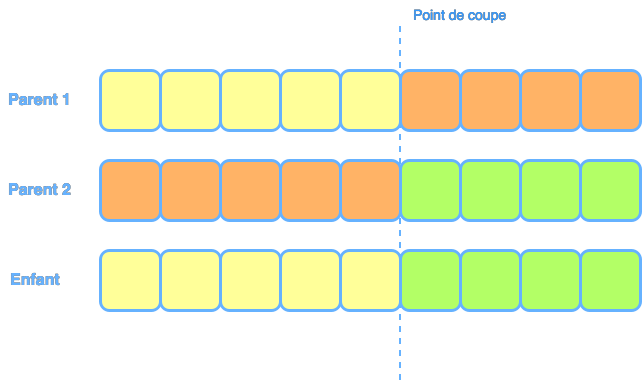
\includegraphics[width=3.5in]{img/crossover.png}
		\caption{Cross-over one point.}
	\end{center}
\end{figure}


\paragraph{BCRC}\label{bcrc}

Pour corriger les problèmes du cross-over mono-point, un
\emph{cross-over} dit \textit{BCRC\cite{ombuki2006multi}} (\emph{Best cost route cross-over}) plus
récent et plus adapté au problème de \textit{ VRP} fut sélectionné pour le
remplacer de mon initiative. N'ayant pas d'implémentation disponible, il
fut d'abord prototypé en \textit{Python} à l'aide du framework évolutionnaire
\emph{DEAP} sur un problème de \emph{VRP} synthétique en utilisant les
jeu de données de VRP standard de Solomon\cite{solomon1987algorithms}. Après validation des
résultats, je l'ai porté en \textit{C++}, non sans difficulté du fait de
son utilisation massive de structure de données dynamique, délicatesse
non permise pour l'architecture \textit{GPU} visée pour des raisons de
performances. \\
Cette implémentation \emph{C++} fut la source de bien des
déboires tant au niveau de l'implémentation que des performances sur
\textit{GPU} du fait de ses nombreuses divergences et de la nécessité
d'allocation mémoire dynamique.

\begin{figure}[htbp]
	\begin{center}
		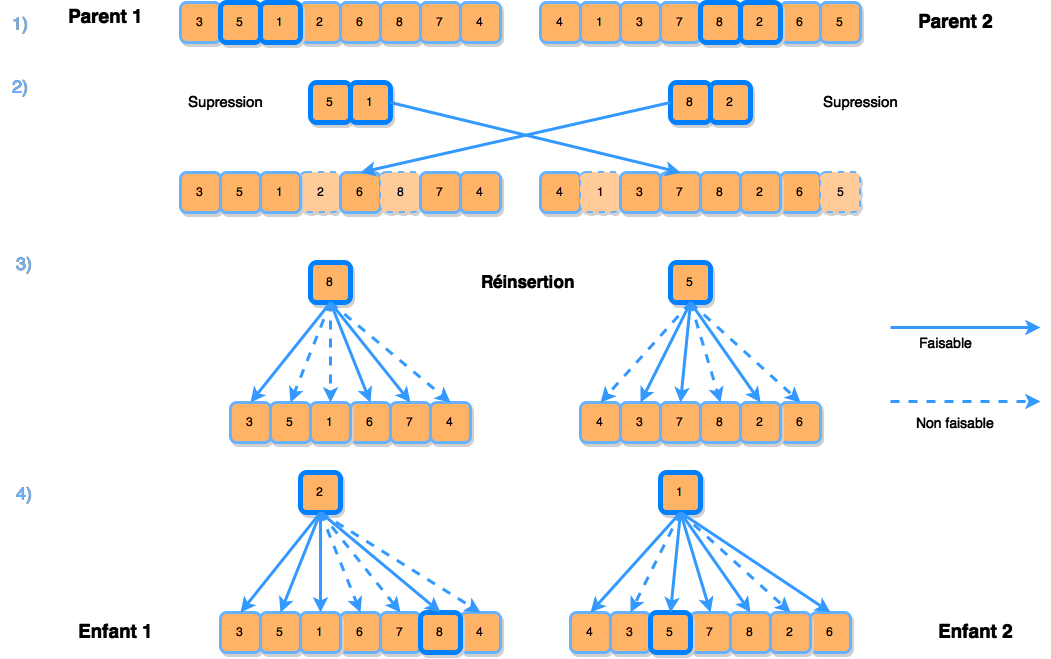
\includegraphics[width=6in]{img/BCRC.png}
		\caption{Best Cost Route Cross-over.}
	\end{center}
\end{figure}

\paragraph{EAX}\label{eax}

Une grande nouveauté dans les techniques de crossover pour les problèmes
de \emph{VRP} fut l'apparition d'\emph{EAX\cite{nagata2006new}}. \emph{EAX} est un crossover
basé sur la recombinaison d'arrêt de graphe (\emph{Edge recombinaison}).
Il permet au GA de rivaliser en qualité avec les autres types de
métaheuristique en particulier les recherches \emph{taboues} pour les
grandes instances de \emph{VRP} (\textgreater{} 30000 « villes »). \\
 Je
m'occuperai de sa mise en place dans le futur, et s'il présente des
avantages concrets en terme d'accélération et de qualité des résultats
obtenus, il remplacera le \emph{cross-over BCRC} actuelle.

\subsubsection{Sélection et ranking : NSGAII et
ASREA}\label{suxe9lection-et-ranking-nsgaii-et-asrea}

Une des grosses avancées de ces dernières semaines est le remplacement
de l'algorithme de sélection \emph{NSGA-II\cite{deb2002fast}} au profit d\emph{'ASREA\cite{sharma2010archived,tsutsui2013massively}}.\\
\emph{NSGA-II} est de facto l'algorithme de \emph{ranking} et de
sélection des \emph{MOEA}, avec une complexité asymptotique en O
(\emph{mn\^{}2}) avec \emph{m} nombre d'objectif et \emph{n} nombre
d'individu. Les implémentations en \emph{C/C++} de \emph{NSGA-II} sont
nombreuses, ce qui a justifié son choix dans un premier temps par M.
Catania.\\
Avec de grandes tailles de populations (\textgreater{}10 000
individus), le temps pris par \textit{NSGA-II} devient significatif par
rapport au reste de l'algorithme. Il se base sur le classement de rang
selon le principe de \textit{Pareto dominance} déjà évoqué plus haut. J'ai donc
décidé d'utiliser \textit{ASREA}, un algorithme de \textit{ranking} par archive
récent et innovant en O (\emph{man}) avec \emph{a} taille de l'archive ,
et sa variante parallélisée sur \emph{GPU}, \emph{G-ASREA\cite{sharma2010gpgpu}}.

\bigskip
\emph{NSGA,} comme \emph{ASREA}, propose une gestion de l'élitisme, le
premier par son classement déterministe de rang et le second par
l'utilisation d'une archive des meilleurs individus. Une explication
plus poussée des deux algorithmes est disponible en annexe. \\
Les accélérations d'\emph{ASREA} et \emph{G-ASREA} sont très
impressionnantes par rapport à \emph{NSGA-II}.
\begin{figure}[htbp]
	\begin{center}
		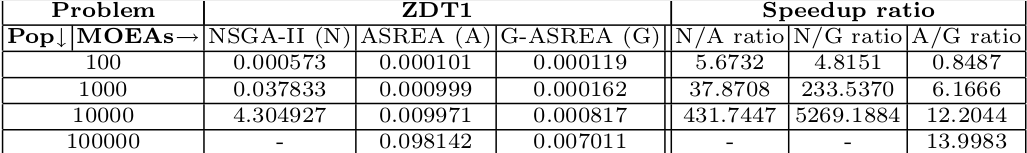
\includegraphics[width=6in]{img/asrea_table.png}
		\caption{Comparaison des temps et accélérations entre ASREA, NSGA-II et G-ASREA sur une minimisation de fonction ZDT\cite{zitzler2000comparison}.}
	\end{center}
\end{figure}
M. Collet m'a fourni une implémentation pour \textit{GPU} d'\emph{ASREA}. Le
code de l'algorithme était fortement imbriqué dans un programme de
benchmarking synthétique de \emph{GA} (\emph{ZDT functions\cite{zitzler2000comparison}}).

Nous avons continuer le travail de parallélisation sur \textit{G-ASREA} pour
qu'il soit exécuter en sont intégralité sur \textit{GPU}. Après extraction,
refactoring et adaptation, nous avons pu bénéficier d'accélérations
répertoriées dans la table suivante :

\begin{center}
	\begin{tabular}{ |l| c| r| }
		\hline
		Nombre d'individu & NSGA-II & G-ASREA \\
		\hline
		1024 & 5 ms & 2 ms \\
		16 384 & 464 ms & 19 ms\\
		32 768  & 1563 ms& 27 ms\\
		\hline
	\end{tabular}
	\captionof{table}{Temps de la sélection, moyennes sur 50 générations.}
\end{center}

\subsection{Implémentation CUDA}\label{impluxe9mentation-cuda}

Tout au long de cette section, la terminologie relative aux technologies
et les technologies elles-mêmes \emph{CUDA} seront explicitées et mises
en perspective avec le développement du projet \emph{HIRONDELLE}.\\
Pour
bien comprendre le modèle de calcul de l'architecture \emph{CUDA}, une
petite explication du modèle \emph{SIMD} et \emph{MIMD} est requise. Ces
modèles de parallélisme sont répertoriés par \textit{la taxonomie de Flynn}.

\begin{figure}[htbp]
	\begin{center}
		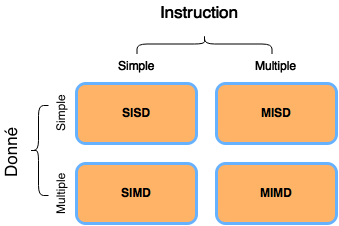
\includegraphics[width=3in]{img/FLYNN.png}
		\caption{Taxonomie de Flynn.}
	\end{center}
\end{figure}

\subsubsection{MIMD}\label{mimd}

\emph{MIMD} (\emph{multiple instruction, multiple data}) est la
technique de parallélisme la plus courante des processeurs modernes. \\
En \emph{MIMD}, les différentes unités de calcul (cœur) peuvent
travailler de manière asynchrone et indépendante sur des données
différentes, \textit{i.e} à un moment \textit{t} donné des instructions différentes sont
effectuées sur des entrées différentes. Cela permet concurrence et
parallélisme au niveau des données. D'un point de vue hardware, la mise
en place d'un tel procédé requiert une architecture complexe et
couteuse, présence de cache, registre et pipeline indépendant pour
chaque unité de calcul et gestion de changement de contexte. Ces
prérequis matériels limitent le nombre d'unités de calcul sur une puce.

\subsubsection{SIMD}\label{simd}

La vision radicalement opposée que propose l'architecture des cartes
\emph{GPGPU} est le modèle \emph{SIMD} (\emph{Single instruction
multiple data)}. Ici, les unités logiques sont nettement moins complexes
et de fait bien plus nombreuses (2880 cœurs sur \emph{NVIDIA titan}).
Une unique instruction est effectuée simultanément sur des entrées
différentes. Cela permet d'exploiter le \emph{data level parallelism},
mais ne permet pas de concurrence. À travers l'utilisation d'algorithmes
adaptés, des accélérations massivement peuvent être atteintes, avec un
ordre de magnitude de plusieurs centaines de fois.

\subsubsection{Architecture software}\label{architecture-software}

\paragraph{Threading model}\label{threading-model}

Le \emph{C CUDA} est une extension du langage \emph{C} (avec une partie
des spécifications du \textit{C++}). Ce métalangage\cite{sanders2010cuda} introduit des
qualifier pour les fonctions et pour les déclarations de variable qui
spécifie quelle partie du code doit être compilée avec le compilateur
\textit{CUDA nvcc} et où elles doivent être exécutées (\emph{host/CPU} ou
\textit{device/GPU}).

\begin{itemize}
\item
  \textbf{global}, depuis l'\emph{host} vers le \emph{device}. Il s'agit
  des \emph{kernels}.
\item
  \textbf{device}, depuis le \emph{device} vers le \emph{device}
\item
  \textbf{host}, depuis l'\emph{host} vers l'\emph{host}
\end{itemize}

\bigskip
Les fonctions qualifiées de \emph{\textbf{global}} sont appelées
\textbf{kernel} : elles seront exécutées n fois en parallèle sur la
carte selon leurs configurations d'appel.\\
Un appel de \emph{kernel} utilise la syntaxe suivante qui définit le
nombre d'exécutions:

\begin{verbatim}
kernel<<< NumberOfBlock,  BlockDimension>>> ( kernel arguments,...);
\end{verbatim}

Chaque thread exécutant un \emph{kernel} se voit attribuer un unique
identifiant relatif à son block, accessible grâce à la variable
built-in \textit{threadIdx}. Le threading model de l'architecture \textit{CUDA}
est pensé pour exploiter au maximum le modèle \emph{SIMD} grâce à une
gestion fine de l'indexage des threads.

\begin{figure}[htbp]
	\begin{center}
		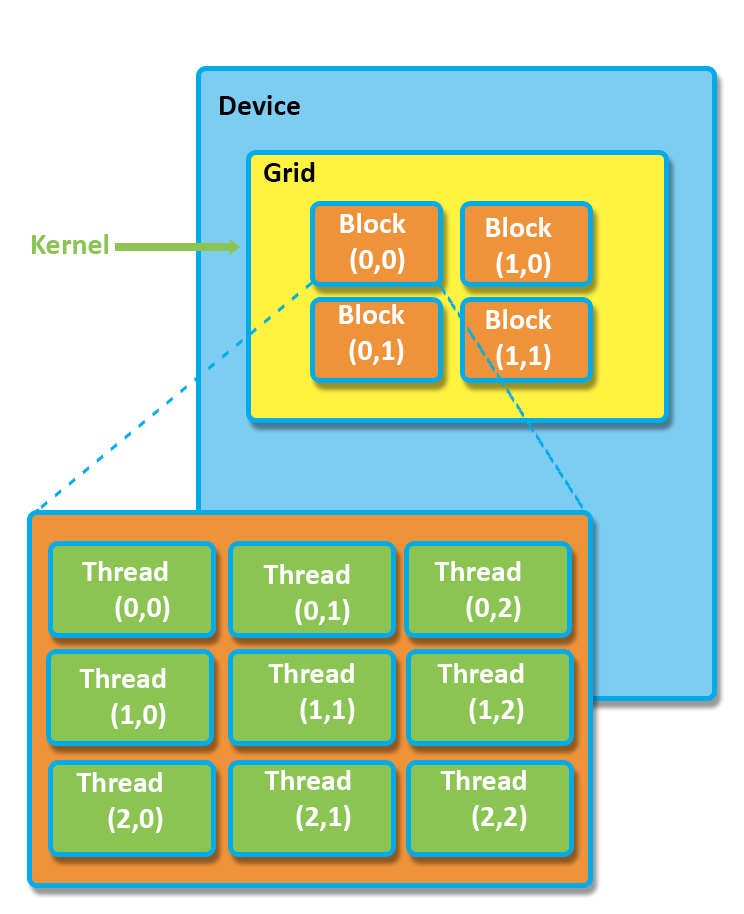
\includegraphics[width=3in]{img/cuda-threading.png}
		\caption{Schéma du modèle de threading de l'architecture \textit{CUDA}}
	\end{center}
\end{figure}

\paragraph{Block}\label{block}
Les \emph{threads CUDA} sont regroupés en \emph{blocks}, eux-mêmes
regroupés sur une \emph{Grid}. Les \emph{threads} ont un unique
identifiant au sein de leurs \emph{blocks}, tout comme chaque
\emph{block} à un unique identifiant au sein d'une \emph{Grid}. Au
niveau des \emph{kernels}, une petite arithmétique d'indexage permet de
calculer des index de tableau continu, pour que chaque thread ne modifie
que des cases mémoire distinctes, pour éviter les « \emph{race condition
}», comme le montre ce court extrait de code:

\begin{verbatim}
int tid = blockIdx.x * blockDim.x + threadIdx.x;
\end{verbatim}


\paragraph{Thread}\label{thread}

Les \emph{threads} d'un même \emph{block} sont exécutés sur un
\emph{multiprocesseur} (\emph{MP}), avec la possibilité de
synchronisation (\emph{barrier}) et de mémoire partagée. \emph{NVIDIA}
définit un autre groupement, plus fin, de \emph{threads} au sein d'un
\emph{block}, appelé \textit{warps}. La gestion de la répartition des
\textit{blocks} sur les multiprocesseurs (physique) est gérée par le
\emph{runtime driver CUDA}, dépendamment du type de \emph{scheduling}
choisie (dynamique, statique, etc...). \\
Selon l'architecture \emph{CUDA}
visée, ``\emph{sm\_compute} 35'' dans notre cas, les limites de nombre
de \emph{block}, de \emph{threads} par \emph{block}, du nombre de
\emph{threads} par \emph{warp} varient. Du fait de regroupement par
\textit{warps}, cela n'a pas vraiment d'intérêt de choisir une taille de
\textit{block} non multiple de la taille des \emph{warp} (qui elle aussi dépend
de l'architecture et du hardware lui-même). L'optimisation \emph{CUDA}
demande donc une connaissance du matériel qui va être utilisé. \\
Voici le tableau des spécifications de la carte \textit{GPGPU} cible, la
\emph{NVIDIA titan}:


\begin{center}
	\begin{tabular}{ |l| c| }
		\hline
Nombre de multiprocesseurs & 15 \\
			\hline
Nombre de coeurs par MP & 192\\
			\hline
Nombre de coeurs total & 2880\\
			\hline
Vitesse d'horloge d'un coeurs & 980 Mhz\\
			\hline
Mémoire global &  6144 MBytes\\
			\hline
Taille des warps & 32\\
			\hline
Nombre de registre 32 bit par block & 65536\\
			\hline
Nombre de thread par block & 1024\\
			\hline
Nombre de thread par MP & 2048\\
			\hline
	\end{tabular}
	\captionof{table}{Spécification de la carte NVIDIA Titan}

\end{center}


\paragraph{Compilation}\label{compilation}

Le \emph{runtime driver CUDA} en lui même est un petit système
d'exploitation : \emph{scheduler}, gestion mémoire et changement de
contexte et plus étonnant même, compilateur \emph{Just-in-time}
(\emph{JIT}). Les évolutions d'architecture étant tellement importantes
et imprévisibles que pour garantir la rétrocompatibilité de code
\emph{CUDA}, les binaires intègrent directement l'assembleur \textit{PTX\footnote{http://docs.nvidia.com/cuda/parallel-thread-execution/}}
intermédiaire.\\
La raison est la suivante: si l'architecture du matériel exécutant le
programme diffère de l'architecture cible à la compilation, le
\emph{runtime driver CUDA} va recompiler tout le code \textit{CUDA} à la volée
au premier lancement de \emph{kernel}. \\
Les temps de compilation avec le compilateur \textit{nvcc} sont relativement
longs, qui se retrouvent être par moment assez désagréable.


\subsubsection{Architecture physique}\label{architecture-physique}

Les \emph{GPU NVIDIA} ont un certain nombre de multiprocesseurs ou
\emph{stream multiprocesseurs} et \emph{stream
processeur} (les 2880 « \textit{cores} »). Les \emph{multiprocesseurs} sont
capables d'exécuter en parallèle des instructions différentes, mais les 
\textit{warps} au sein de \emph{block} de \textit{thread} exécutent une seule
instruction simultanément au travers d'un modèle \emph{SIMD} modifié, le
\emph{SIMT} (\emph{Single Instruction, multiple Thread}). 

\bigskip
Le modèle \emph{SIMT} est capable de gérer les branchements
conditionnels en désactivant dynamiquement les cœurs exécutant des
branches différentes, pour faciliter le travail du développeur. Cela
entraîne une baisse de performance appelée divergence, dons nous
discuterons dans les sections suivantes.

\subsubsection{Hiérarchie mémoire}\label{hiuxe9rarchie-muxe9moire}

\begin{figure}[htbp]
	\begin{center}
		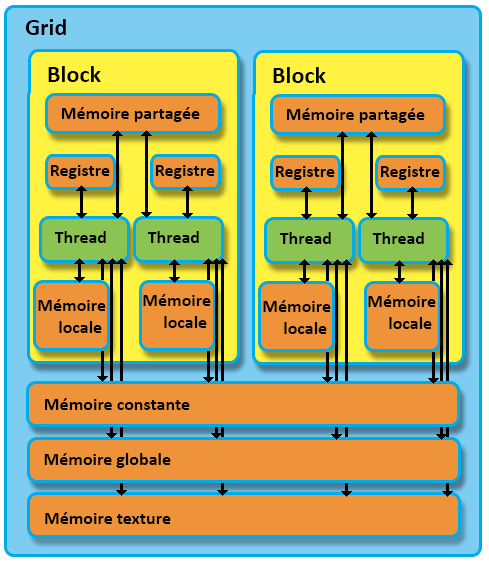
\includegraphics[width=3.3in]{img/cuda_memory.png}
		\caption{Les différents type de mémoire de l'architecture \textit{CUDA} et leurs portées.}
	\end{center}
\end{figure}

La hiérarchie mémoire de la plateforme \emph{CUDA} est assez simple si
ce n'est un peu long. Ici ne seront donnés que les points clés pour
aider à la compréhension du lecteur. Il y a six types logiques de
mémoire différente correspondant à plusieurs zones mémoire physiques
différentes :

\paragraph{Globale}\label{globale}

Les accès à la mémoire globale de type \emph{DRAM} sont lents, et ce
malgré un système de \emph{cache} hardware. C'est le type de mémoire le
plus important en capacité. \\
La plupart des accès mémoire dans hirondelle réfère à la mémoire globale
malgré les efforts répétés d'utiliser convenablement les autres. Y sont
présentes les données du problème ainsi que les différentes populations
d'individu.

\paragraph{Constante}\label{constante}

La mémoire constante stocke les arguments des \emph{kernels} (appel de
fonction sur le device) et les valeurs constantes définies avec le
mot-clé spécial \textit{\_\_constant\_}. Elle est particulièrement petite et
nous n'en avons pas d'utilité. Elle est cependant particulièrement
rapide.

\paragraph{Texture}\label{texture}

La mémoire des textures est un peu différente de par son accession en
2D. Elle serait donc particulièrement adaptée à notre cube.

\paragraph{Partagée (shared)}\label{partaguxe9e-shared}

Le mécanisme principal de communication entre threads est d'utiliser la
mémoire partagée. Partagée dans le sens ou tous les \emph{threads} d'un
\emph{block} y ont accès. Elle est particulière rapide, quoique limitée
en capacité (seulement \emph{64k} pour la titan) et organisée sous forme
de \emph{bank} retournant des \emph{words} de 32 \emph{bit}. L'accès a
un même words en simultané résulte en un \emph{bank conflict}. \\
Les
\emph{patterns} d'accès suivant sont possibles:

\begin{itemize}
\item
  Accès simple chaque \emph{thread} demande d'un mot d'une \textit{bank}
  différentes
\item
  Accès \textit{broadcast}, tous les \textit{threads} d'un même \emph{warp}
  demandent un mot d'une même \emph{banks}
\end{itemize}

\bigskip
Un \textit{bank conflict} provoque la sérialisation des accès mémoires
impactant les performances.

\bigskip
La technique de \emph{tiling} couramment utilisé pour les programmes
limités par l'utilisation mémoire plutôt que par les opérations
arithmétiques est de découper les données à utiliser en \emph{tile} de
\emph{64k}. \\
Dans notre cas cela n'est malheureusement pas possible, dû à l'empreinte
mémoire des individus qui prendrait l'intégralité de la mémoire partagée
de chaque bloc. Cela résulterait en une exécution en parallèle du nombre
de \emph{MP} disponible soit 16 pour la titan black.

\paragraph{Registre}\label{registre}

Chaque \emph{stream multiprocessor} en plus de la mémoire partagée est
aussi composé de 32 768 registres de 32 \emph{bits}. Les registres ne
sont pas partagés entre les \emph{threads}. Les registres correspondent
à la mémoire la plus rapide embarquée sur les cartes \emph{GPGPU NVIDIA}
et servent à stocker les variables locales de chaque \emph{thread} et
les résultats des opérations de base à la manière des registres
\emph{CPU}. Si la taille des variables locales excède le nombre de
registres alloué à un \emph{thread}, celles-ci sont automatiquement
placées dans la mémoire locale impactant significativement les
performances, dans un processus appelé ``\emph{spilling\cite{sanders2010cuda}}''. 

\bigskip
Ainsi, mettre trop de \emph{threads} par \emph{block} résulte en un
nombre de registres limité pour chacun d'entre eux et limite
possiblement les nombres de tâches exécutables simultanément,
dépendamment des variables locales déclarées et du nombre d'opération
arithmétique concurrente.\\
Un soin spécial a été apporté pour réduire le nombre et la taille des
variables locales des différents \emph{kernels}. Le \emph{flag} du
compilateur \emph{nvcc ptxas-verbose} indique les \emph{spills} et tout
comme les rapports du profileur \emph{nvprof} fournit dans le \emph{sdk
CUDA}.

\subsubsection{Optimisation et détails
d'implémentation}\label{optimisation-et-duxe9tails-dimpluxe9mentation}

\paragraph{Appel coalescent}\label{appel-coalescent}

L'appel de mémoire coalescent est une technique pour augmenter
l'utilisation de la bande passante de la mémoire globale en «
\emph{coalesçant }» (groupant) les transactions d'accès mémoire. Cela
est possible quand les \emph{threads} au sein d'un \emph{demi-warps}
accèdent en parallèle à des zones mémoire consécutives. Le \emph{driver
CUDA} va alors grouper les transactions pour récupérer des \emph{words}
d'une taille de 64 ou 128 \emph{bits} réduisant considérablement la
latence d'appels mémoires global, particulièrement lent (600-800
cycles). \\
Il s'agit du gros point noir du projet, car les accessions
mémoires sont par nature aléatoires vu le processus stochastique
évolutionnaire. Les \emph{patterns} d'accès à la mémoire globale sont
donc particulièrement aléatoires, et résiste à tout type d'analyse
statistique. Généralement des techniques de \emph{tiling} sont utilisées
pour réduire les latences mémoire en découpant les données globales en
bloc de \textit{64k} et en les plaçant dans la \textit{shared memory}, qui n'a quasiment
pas d'\emph{overhead} (la mémoire partagée des blocks correspond au
cache L1 directement placé sur les puces des \emph{multiprocesseurs}).

\bigskip
Malheureusement, les volumes de données utilisés nous empêchent là
encore d'utiliser ce type de mémoire. Une technique envisagée est le
prétraitement des données globales avec chaque appel de \emph{kernel}.
Cela consiste à regrouper des individus référençant des données
similaires et en créant des \emph{subsets} des données globales
correspondant à ces groupes d'individu. \\
Mais là encore, le nombre de données à utiliser et la distribution quasi
uniforme (du moins dans les premières générations) des références des
individus rendent ce type d'optimisation

\begin{figure}[htbp]
	\begin{center}
		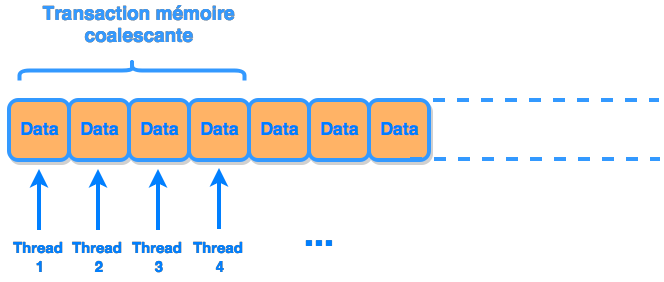
\includegraphics[width=4in]{img/coalescent.png}
		\caption{Transaction mémoire coalescentes.}
	\end{center}
\end{figure}

\begin{enumerate}
\def\labelenumi{\arabic{enumi})}
\item
  particulièrement ardu à implémenter efficacement
\item
  fort probablement une anti-optimisation si les préconditions ne
  peuvent être remplis, \textit{i.e} aucun \emph{subset }possible inférieur à la
  limite de \textit{64k} de la mémoire partagé ce qui entraînerait
  l'utilisation de la mémoire globale comme \emph{fallback}.
\end{enumerate}

\paragraph{Divergence}\label{divergence}

L'architecture matérielle des cartes \emph{GPGPU CUDA }requiert que les
\textit{warps} (ou les \emph{half-wrap} pour l'architecture Fermi) suivent la
même trajectoire, \textit{i.e} exécutent exactement les mêmes instructions donc
les mêmes branchements. Pour le modèle \emph{SIMD}, les \emph{threads}
ne peuvent théoriquement pas diverger.\emph{NVIDIA} propose ici une
solution pour les branchements conditionnels types \textbf{if-then-else} et
autres boucles au nombre d'itérations variable. Les threads évaluant la
partie \textbf{then} se retrouvent à exécuter des instructions
différentes des threads évaluant la partie \textbf{else}. 

\bigskip
La plateforme \emph{CUDA} propose un contournement du problème, qui
impacte néanmoins les performances. Dans le cas de
l'\textbf{if-then-else}, pendant qu'une partie des \emph{thread}s évalue
la partie \textbf{then}, ceux devant évaluer le \textbf{else} sont
désactivés et vice-versa, sérialisant de facto une partie des
traitements parallèlesLe traitement des nombreuses contraintes dans la
fonction d'évaluation de pair avec les différences au niveau des données
des individus résulte dans une grande quantité de divergences,
visualisable grâce à l'outil de profiling \emph{nvvp} et \emph{nvprof}.
\emph{Nvvp} donne une analyse point par point des problème et
\emph{hotspot} de chaque \emph{kernel}. \\
Plusieurs mécanismes ont été utilisés pour réduire le nombre de
divergences sans trop changer la logique :

\begin{itemize}
\item
  Arithmétisation de conditionnel
\item
  Découpage en \emph{sous-kernel}
\end{itemize}

\bigskip
L'arithmétisation de conditionnelle consiste à transformer un
branchement conditionnel en opération arithmétique. Ici un simple
exemple fera foi :

    \begin{figure}[ht]
    	\begin{minipage}[b]{0.5\linewidth}
    		\centering
    		\begin{verbatim}
    		int val = 0;
    		
    		if(foo)
    		    val += 500;
    		else
    		    val+= 250;
    		\end{verbatim}
    		\caption{Extrait de code divergent}
    	\end{minipage}
    	\hspace{0.5cm}
    	\begin{minipage}[b]{0.5\linewidth}
    		\centering
    		\begin{verbatim}
    		int val = 0;
    		
    		val += 250 + (foo * 250);
    		\end{verbatim}
    		\caption{Version "arithmétisé"}
    	\end{minipage}
    \end{figure}

\bigskip
Le découpage en sous-kernel reste la technique la plus simple à mettre
en place. \\
Les gros \emph{kernels} très divergents sont découpés fonctionnellement
en plus petit sous-kernel. Comme toute optimisation et à cause de la
complexité des mécanismes et procédures en jeux, les \emph{hotspots} se
détectent uniquement par l'utilisation de \emph{profiler}. \\
Sacrifier de
la lisibilité pour des gains de performance nuls ou négligeables n'as
pas de sens.

\begin{figure}[htbp]
	\begin{center}
		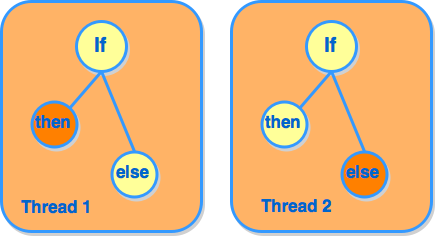
\includegraphics[width=3in]{img/divergence.png}
		\caption{\textit{Divergence}: Deux threads executant un branchement différent.}
	\end{center}
\end{figure}



\subsubsection{Futurs développement et interaction
utilisateur}\label{futurs-duxe9veloppement-et-interaction-utilisateur}

Nous allons donc procéder en trois temps:
\begin{itemize}
\item
  Intégration et test de l'optimisation pour le lendemain, statique
\item
  Optimisation statique et gestion des ajout et délétion de mission par
  un algorithme annexe de recherche locale
\item
  Optimisation entièrement dynamique anytime par l'algorithme génétique
  lui-même
\end{itemize}

\bigskip
Nous allons ajouter la visualisation des équipages et leurs assignations
sur Saphir, pour pouvoir monter des plannings à des planificateur et
régulateur le plus tôt possible. Cela nous permettra de corriger les
gros problèmes, dont les éléments et contraintes manquants. \\
J'ai proposer de mettre en place une méthodologie de test en aveugle (et
si possible en double aveugle) pour voir si les régulateurs sont
satisfaits des plannings proposés et s'il les différencie d'un planning
fait par un humain compétent. \\
Au niveau de l'interaction avec le décideur, il devra choisir un
planning parmi un front de Pareto, sur le front lui-même ou à travers de
slider pour sélectionner des plannings optimisant plutôt les coûts ou la
qualité de service. On y affichera aussi des statistiques simples pour
chaque planning: coût, retard cumulé, nombre de véhicules utilisé,
nombre d'employées utilisé, ect \ldots{}

\bigskip
J'ai aussi proposé un côté interactif, en permettant aux régulateurs de
``bloqué'' des parties qui leur semblent intéressantes. Nous pouvons
gérer de cela manière génétique, en assignant un bonus à l'évaluation
aux individus incluant ces bloques de mission figée ou de manière plus
déterministe, plus agréable et facile à suivre pour l'utilisateur, mais
offrant potentiellement de moins bonnes optimisations futures dues à
l'ajout de contraintes. Des études futures sur la fatigue utilisateur,
courante dans le domaine des optimisations interactives\cite{cho2002towards} par algorithme
génétique doivent encore être conduites. \\
Pour toute la partie dynamique, les véhicules en cours de mission
doivent être considérés comme utilisés jusqu'à leurs prochaines missions
planifiées, le reste de l'optimisation devant continuer avec ces
nouvelles contraintes. Ce fonctionnement demande une observation sur le
terrain de la réaction des régulateurs, car ils perdent une partie de
leurs contrôles sur la planification au profit de l'algorithme.

\subsubsection{Résultats
expérimentaux}\label{ruxe9sultats-expuxe9rimentaux}

Nous avons obtenu de bons résultats concernant le nombre de véhicules
utilisés par rapport au nombre de missions, en des temps plus que
corrects. Nous utilisons uniquement des données réelles de journée déjà
passée, fournies par les bases de données de Saphir. \\
Ces résultats ont été validés par des professionnelles de la régulation
de transport sanitaires et sont corrects dans le sens où ils respectent
les contraintes légales et logistiques fortes (pas de simultanée pour
les ambulances, présence de pause d'au moins 20 minutes toutes les 6
heures, ect .. ). \\
Ici nous pouvons voir représentation graphique sous forme de Timeline
des missions à effectuer pour chaque véhicule.

\begin{figure}[htbp]
	\begin{center}
		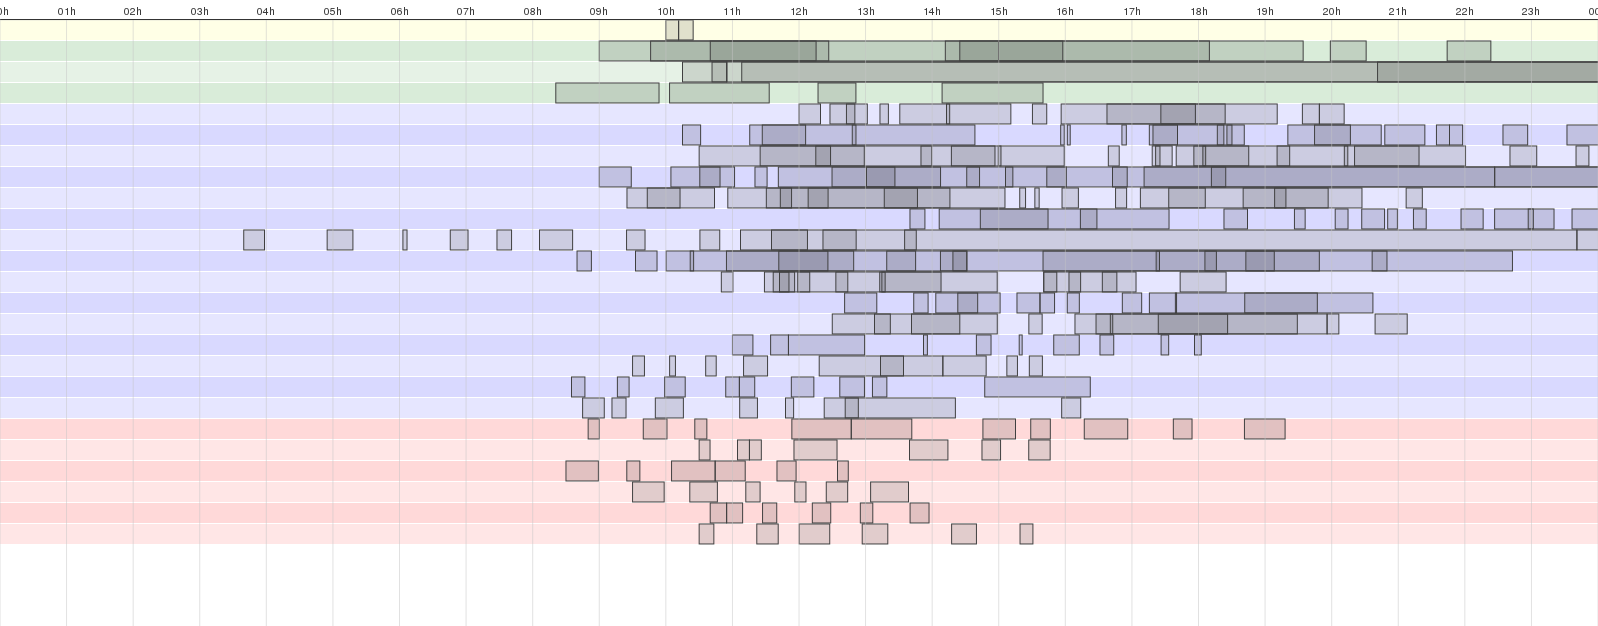
\includegraphics[width=6in]{img/hirondelleTimeline.png}
		\caption{\textit{Planning:} Chaque ligne correspond au mission d'un véhicule sur une journée. En rouge les ambulances, en bleu les taxis, en vert les VSL et en jaune les TPMR.}
	\end{center}
\end{figure}

D'un point de vue des temps de calcul, nous sommes satisfaits des
valeurs obtenues. J'ai répertorié ici les différentes accélérations
observées entre la version CPU séquentielle et la version GPGPU
massivement parallélisée de notre implémentation:

\begin{center}
	\begin{tabular}{ |l| c| r|}
		\hline
Implémentation &Milliseconde par génération &Accélération sur CPU \\
\hline
CPU single threaded & 1566 &1x\\
\hline
GPU Debug&  534 & 2,8x \\
\hline
GPU Release& 44 & 34,8x \\
\hline
	\end{tabular}
	\captionof{table}{Pour une population de 16 384, moyennes sur 40 générations.}
\end{center}


Il est cependant important d'admettre que les accélérations sur GPU
pourraient être un ordre de magnitude supérieur\cite{pospichal2010parallel}, notre implémentation
étant exécutée dans son intégralité sur GPU. La loi d'Amhdal\cite{hill2008amdahl} définit que
l'accélération théorique maximale dépend du temps passé sur les parties
séquentielles du programme, quasi nulle dans notre cas:

\bigskip
\textbf{Soit}
\begin{itemize}
\item
 $ n \in I\!R$, le nombre de thread disponible,
\item
  $B\in [0, 1]$, La fraction du programme strictement séquentielle
\end{itemize}

\bigskip 
Le temps $T \left(n \right)$ pour que le programme finisse son exécution
avec \textit{n} threads:\\

$T(n) = T(1) \left(B + \frac{1}{n}\left(1 - B\right)\right)$

\bigskip
L'accélération théorique maximale S(n) dépend donc de \\

$S(n) = \frac{ T\left(1\right)}{T\left(n\right)} =
\frac{T\left(1\right)}{T\left(1\right)\left(B + \frac{1}{n}\left(1 - B\right)\right) }
= \frac{1}{B + \frac{1}{n}\left(1-B\right)}$

\bigskip
Au niveau de la gestion des employés, nos résultats sont en deçà des
fourchettes fournies par les régulateurs ambulanciers. Notre
optimisation nous donne \textasciitilde{}60 employées pour 250 missions
alors qu'on devrait obtenir entre 40 et 45. De grandes améliorations de
cette partie de l'algorithme sont en cours de développement.

\begin{figure}[htbp]
	\begin{center}
		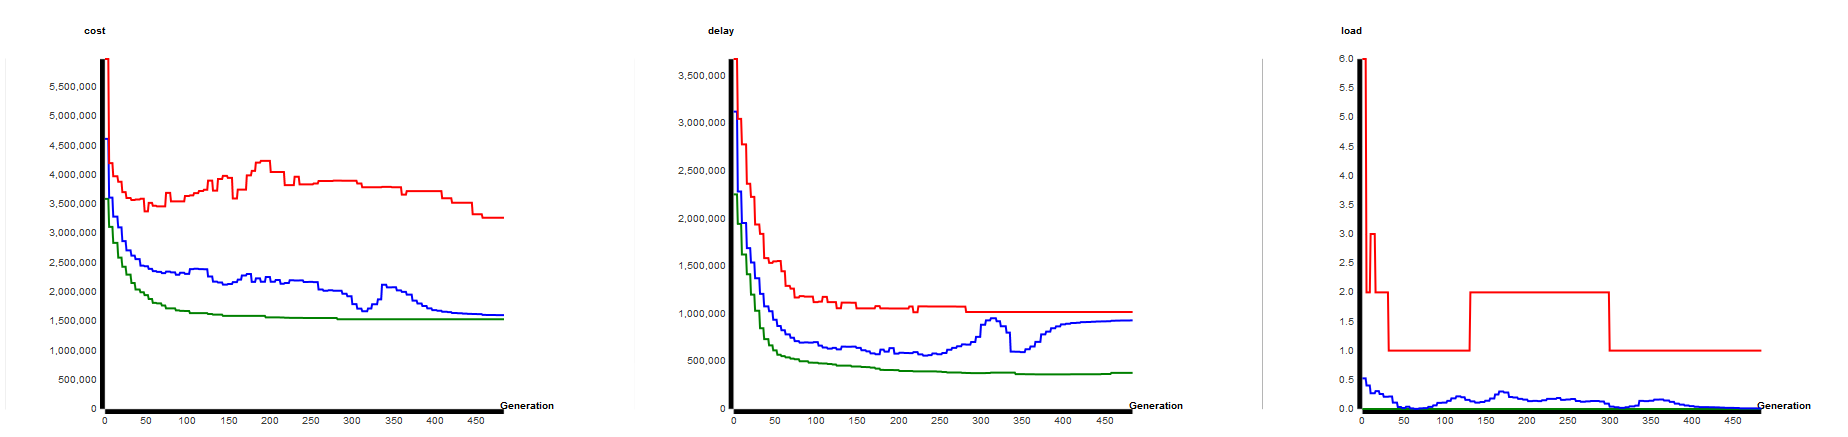
\includegraphics[width=6in]{img/stat}
		\caption{L'évolution des différentes fitness sur 1000 générations. De gauche à droite, la fitness de coût, de retard cumulé et de capacité. Pour chaque objectif, en rouge la pire valeurs de fitness de la population, en bleu la fitness moyenne et en vert la meilleurs.
	    Machine: NVIDIA Titan, core i5 2500K, 12GB DDR3 avec une taille de population de 1024 individus.}
	\end{center}
\end{figure}

\subsection{Gestion de projet et capacité
d'adaptation}\label{gestion-de-projet-et-capacituxe9-dadaptation}

De mon poste au \emph{CNRS} à ma position actuelle d'assistant-chercheur
à \emph{Synovo}, j'ai joui d'une certaine indépendance et liberté dans
la manière dont lesquels les projets étaient pilotés. Les finalités des
différents projets auquel j'ai participé n'étant pas les mêmes, les
prises de décisions sur des questions techniques et conceptuelles ainsi
que les modalités de rendu différaient grandement. J'ai travaillé dans
divers environnements: seul, en collaboration ponctuelle et en équipe.
Je gère à présent une équipe de deux personnes au bout de quelques mois
chez \emph{Synovo}, ce qui m'a beaucoup apporté sur le plan
professionnel et personnel, sur des questions auxquelles je ne me suis
jamais retrouvé confronté auparavant. \\
Nous passerons en revue dans les
prochaines sections tour à tour ces expériences, et l'apprentissage qui
ont été tirés de chacune d'elle et de leurs influences. Nous tâcherons
aussi de mettre en lumière les différences de fonctionnement et
d'attente entre la recherche dans le monde universitaire et le secteur
privé.

\subsubsection{Autonomie et capacité
d'adaptation}\label{autonomie-et-capacituxe9-dadaptation}

Dans les projets énoncés, la plus grande part de responsabilité vient du
fait d'être capable de s'adapter rapidement aux demandes et de pouvoir
proposer des solutions viables peu couteuses en temps-homme. Cette
responsabilité s'accompagne de la capacité à faire de la veille
technologique et à comprendre rapidement le fonctionnement de nouvelles
\emph{bibliothèques, frameworks, langages} et algorithme. \\ 
De la mise en
place d'un système de déploiement à la collecte de données et traitement
statistique en passant par de la visualisation, j'ai été amené à
découvrir beaucoup de domaines de l'informatique qui m'étaient
jusqu'alors mal connus et flous. Cela m'a permis d'acquérir rapidement
une culture générale qui me permet de réagir plus précisément aux
nouveaux problèmes rencontrés.\\
Comprendre et exploiter efficacement une nouvelle technologie requiert
de la discipline et de la concentration : lire de la documentation,
analyser la philosophie sous-jacente et faire une expertise des
limitations du système. Intégrer une solution à un projet déjà existant
reste une problématique à part entière : il faut modifier l'architecture
du projet en conséquence. L'intégration de la partie CUDA sur le projet
\emph{HIRONDELLE} en est un excellent exemple. Le système de build a dû
être grandement remanié, pour bien séparer les parties de code destinées
à l'exécution sur \emph{GPU}. Une nomenclature spécifique de la
hiérarchie de fichier et des directives de compilation
(\emph{preprocessing}) se sont révélées être indispensables. Toutes ces
considérations, que l'on a parfois tendance à mettre de côté, demandent
un véritable travail d'assimilation. \\
Une bonne connaissance des
technologies du Web et les diverses techniques et bonnes pratiques
acquises au travers de projet personnel m'ont obligé à m'interroger sur
le fonctionnement du modèle \emph{MVC} de \emph{Django} et de manière
plus large aux interactions client-serveur basées sur \textit{API RESTful} et
\emph{Ajax}.\\ Tout en approfondissant ma compréhension du langage
\emph{Python}, je me suis aussi familiarisé avec des concepts plus
généraux des langages dynamiques et faiblement typés. Ce n'est qu'au bout
d'un mois que j'étais capable de produire avec aisance du code Python
propre et standard. Une fois la philosophie Python assimilée,
l'utilisation et la découverte de bibliothèques tierces se sont révélées
bien plus faciles.

\subsubsection{Chef d'équipe}\label{chef-duxe9quipe}

Au cours du mois de juin, deux nouveaux développeurs m'ont rejoint sur
le projet HIRONDELLE, Benjamin Chetiou, qui rentre au master ILC en
septembre et Ivan Aksamentov, étudiant au cursus master ingénierie en
informatique de l'université de Strasbourg. \\ Je me suis chargé de leur
faire découvrir le projet et ses enjeux, notamment sur la partie
scientifique et sur les techniques évolutionnaires. Savoir transférer
efficacement ses compétences et connaissances reste pour moi un point
primordial d'une collaboration efficace. Il n'y a pas eu besoin de
formation particulière sur la partie technique de par leurs
connaissances préalables en C/C++, JavaScript et Python.\\
Dans le travail en équipe, il ne faut surtout pas perdre de vue la
dimension humaine. En tant que chef d'équipe c'est de mon ressort de
bien comprendre les compétences techniques et de relation humaine de
chacun pour offrir une ambiance de travail agréable, épanouissante et
productive pour tous. Une petite présentation de l'équipe et de leurs
travaux s'impose. M. Ivan Aksamentov possède une excellente maitrise du
\emph{C++} et de ses spécifications récentes ( \textit{C++11} et \emph{C++14)}. \\
J'ai beaucoup appris de lui sur les idiomes de programmation du langage
C++ comme RAII, pImpl, des concepts de software design orienté objet
diamond problem et des méthodologies de développement comme YAGNI\footnote{"You aren't gonna need it"} ainsi
que sur certains outils et méthode de développement C++ : sanitizer,
mode débug pour la STL\footnote{C++ Standard Template Library} et test unitaire. \\
Mon autre collègue est M.
Benjamin Chetiou. Il a par plusieurs occasions fait preuve d'une grande
capacité de compréhension et de résolution de problème. Il s'occupe de
l'intégration de l'algorithme à \emph{Saphir} et du protocole d'échange
de donnée entre eux. Il s'occupera avec moi de la gestion de la
dynamicité de l'optimisation, requérant des interactions de type
\emph{CRUD\footnote{Create, Read, Update and Delete}} entre le serveur et l'algorithme et la gestion des
équipages.

\subsubsection{Premier pas}\label{premier-pas}

Une fois endossé ce rôle de chef d'équipe, le premier obstacle que j'ai
rencontré est le découpage et la répartition des tâches selon les
compétences et abilitésagilité de chacun. Le fait d'avoir travaillé seul
sur le projet m'a permis d'avoir une vision d'ensemble sur le futur des
développements. S'agissant d'une nouvelle expérience de gestion de
projet dans le cadre professionnelle, je n'avais pas prévu de tâches
assez importantes et je me suis retrouvé au bout d'une semaine sans
tâches précises à distribuer. Je me suis mis à chercher des conseils
auprès de mon supérieur hiérarchique directe, M Guillaume Philips et de
connaissances qui ont été dans la même situation, qui sont elle aussi
passé de développeur à chef de projet. Je me suis permis de tester
différentes approches dans le management au cours des quelques semaines
qui ont suivi, en essayant de mettre en place des méthodologies de
gestion de projet comme \emph{pomodoro\footnote{https://fr.wikipedia.org/wiki/Technique\_Pomodoro} }ou \emph{kanban\footnote{\url{https://fr.wikipedia.org/wiki/Kanban}}}. \\
Cette première
phase s'est révélée un peu tâtonnante, mais extrêmement enrichissante.
Cela est encore plus vrai dans le cadre de la R\&D, où l'on rencontre
parfois des phases de doute et de stagnation. Il s'agit aussi de faire
preuve d'optimisme tout en restant réaliste, ce qui est malheureusement
de mes faiblesses, \textit{i.e} annoncer des délais de mise en production
beaucoup trop courts.

\subsubsection{Difficultés}\label{difficultuxe9s}

Au début, j'avais du mal à jongler entre mes propres taches et la
gestion de projet, écart qui s'est peu à peu réduit avec l'expérience et
l'habitude. Avant de trouver cet équilibre, la responsabilité et la
charge de travail supplémentaire se sont traduites par un certain
stress. Les nombreux interblocages dans les tâches assignées
n'aidaient pas à cela. \\
Je cherche toujours à avoir le feedback des
personnes travaillant avec moi dans le but d'avoir des relations de
travail les plus saines possible. Une bonne ambiance entraîne de
nombreux avantages dont la prise d'initiative et les échanges de points
de vue sur les choix et positionnement architecturaux, conceptuels et
techniques. Ainsi dès qu'une difficulté survient, un processus ouvert de
résolution est enclenché, où chacun confronte ses idées et solutions.

\newpage
\section{Conclusion}\label{conclusion}

Cette première année d'alternance fut riche et dense en expériences. \\
D'un point de vue personnel, j'ai pu fréquenter deux milieux aux buts et
objectifs différents. Par le contact et la présence de nombreux
collaborateurs sur des projets éloignés, j'ai pu me forger une éthique
et des méthodologies de travail flexible et efficace. \\
J'ai dû faire face à des obstacles importants, sur les plans théorique
et technique tout autant que personnel et moral, ce qui m'a permis
d'apprendre à mieux gérer mon stress et de mieux m'en prévenir. J'ai
acquis des démarches et méthodes de résolution de problème plus
rationnelles et professionnelles. \\
L'apprentissage ``\emph{sur le tas}'' de la gestion de projet et
d'équipe enrichie aussi grandement mon bagage en tant que personne et
travailleur. Devenir un bon chef de projet est difficile et faire ses
premiers pas et balbutiements en tant qu'étudiant en alternance permet
d'expérimenter dans un environnement plus facile. \\
Même si déjà exposé superficiellement dans le passée à la programmation
Web et au développent sur \emph{GPGPU}, c'est grâce aux projets auxquels
j'ai eu le plaisir de participer que je suis maintenant pleinement
capable de les maîtriser. J'ai techniquement bien évolué : clarté du
code, rapidité, mise en place de méthodologie de test. L'exposé du
travail effectué tout au long de l'année peut sembler hétéroclite et
même parfois confus, car de nombreuses et diverses tâches m'ont été
confiées.

\bigskip
J'ai particulièrement aimé mon travail sur \emph{EASEA-CLOUD} et
\emph{HIRONDELLE}, tous deux en relation avec les algorithmes
génétiques, qui se trouve être un de mes centres d'intérêt en
informatique. De plus, j'ai toujours fait attention aux questions de
performance, soit le coeur de ces deux projets.\\
Les nouvelles possibilités qu'offrent les solutions de calcul
massivement parallèle \emph{low-cost} dont font partie les cartes
\emph{GPGPU} sont très intéressantes à explorer. \\
Avec la plateforme \emph{EASEA} et sur le projet \emph{HIRONDELLE}, il a
été possible d'utiliser à leurs pleines mesures la puissance de calcul
de cartes \emph{GPGPU NVIDIA} musclées, résultant en des accélérations
convenables (x30 dans le cas d'\emph{HIRONDELLE}) voire impressionnantes
(x400 sur benchmarks avec EASEA\cite{maitre2012easea}). \\
Cela a été rendu possiblement par le parallélisme massif inhérent des
techniques évolutionnaires. Ces accélérations nécessitent d'utiliser des
tailles de population massive, plus de 30000 individus alors que la
plupart des optimisations par algorithme génétique classique requièrent
des populations de 100 à 1000 individus. \\
Cela est dû au fonctionnement de carte \emph{GPGPU}, qui du fait de
leurs architectures physiques simples et du modèle \emph{SIMD} qu'elles
implémentent, demande de ``charger'' les exécutions avec de très
nombreuses tâches pour simuler un système de pipelining, ces cartes
n'ayant pas de scheduler matériel\cite{sanders2010cuda}.\\
Il a été très intéressant de mettre en perspective mon travail sur 
\textit{EASEA-CLOUD}, un framework évolutionnaire et \textit{HIRONDELLE}, une
implémentation très spécifique d'un problème précis. L'utilisation
d'\textit{EASEA-CLOUD} a considérablement réduit le temps de développement pour
avoir un premier prototype au détriment des performances, ce qui est
tout le contraire du développement d'\emph{HIRONDELLE}.

\bigskip
Avoir abordé les deux angles m'a grandement aidé à acquérir une vision
plus complète du domaine de l'optimisation par algorithmes génétiques
autant sur la théorie que sur les détails d'implémentation.

\nocite{*}
\bibliographystyle{plain}
\bibliography{mémoire}

\end{document}
